\chapter{圆锥曲线}

\noindent
\begin{minipage}{.55\textwidth}
    \CTEXindent
   一条直线，绕与其斜交的一条直线旋转一周所形成的曲
面叫做圆锥面. 用不经过这两直线的交点的平面去截圆锥面，可以得到四种交线：圆、椭圆、抛物线和双曲线（图3.1）．这四种曲线统称为圆锥曲线. 

本章将用代数的方法研究它们. 首先推导它们的标准方程，然后研究它们的图形、几何性质及简单的应用.
\end{minipage}\hfill
\begin{minipage}{.45\textwidth}
    \centering
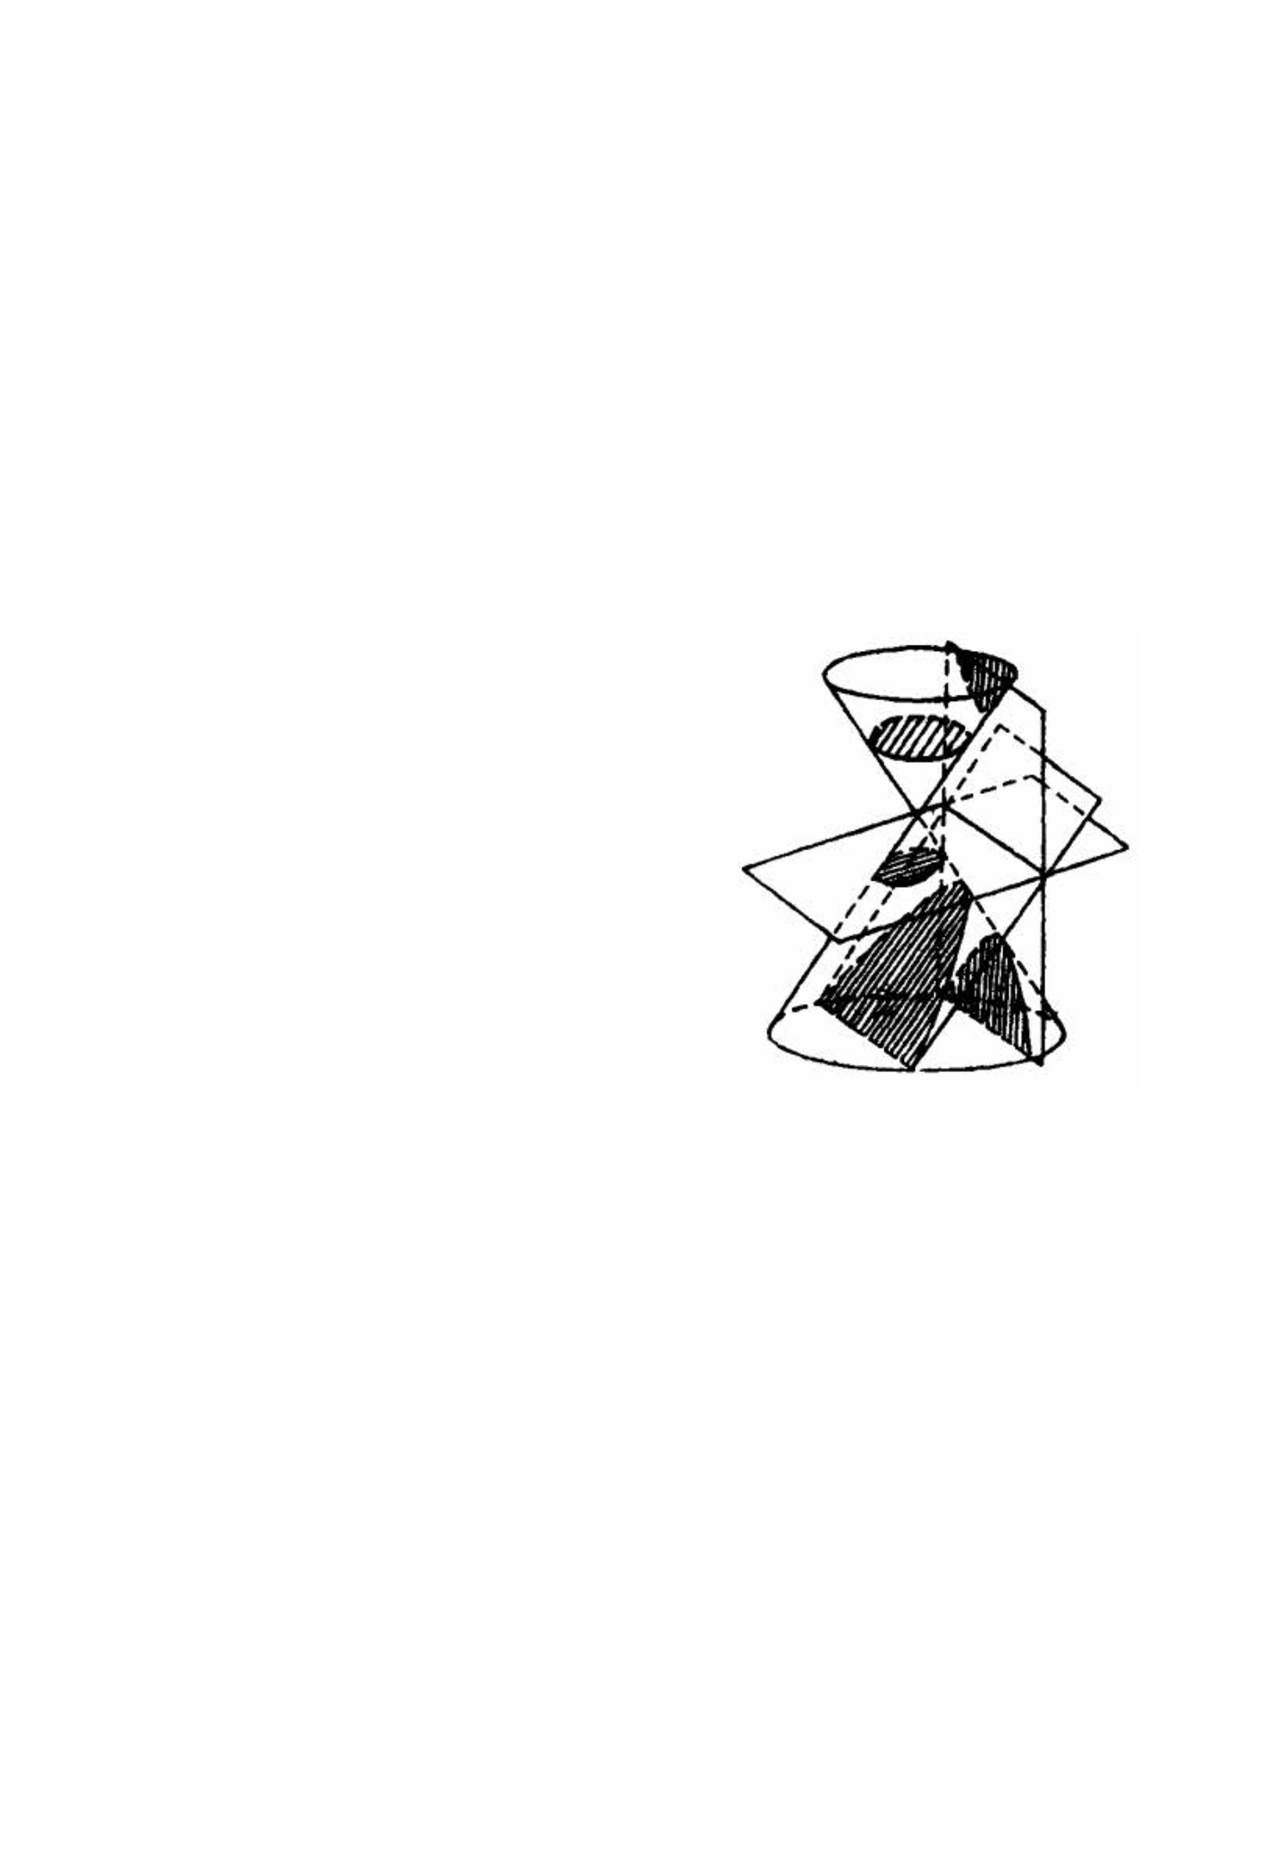
\includegraphics[scale=.6]{fig/3-1.pdf}
\captionof{figure}{}
\end{minipage}



这四种曲线是我们日常生活中
除直线外，接触最多的曲线，它们和天体运行轨道有密切的关系，在科学技术上具有十分重要的地位，是平面解析几何的重要内容.

\section*{一、圆}

\section{圆及其方程}


\noindent
\begin{minipage}{.55\textwidth}\CTEXindent
    平面内到定点的距离等于定长的点的集合（轨迹）叫做\textbf{圆}. 定点叫做圆的\textbf{圆心}，定长叫做圆的\textbf{半径}. 圆上任一点$P$所具有的特征性质就是它到圆心$C$的距离始终等于圆的半径$r$（图3.2）．现在，根据圆的特征性质导出圆的方程.
\end{minipage}
\hfill
\begin{minipage}{.4\textwidth}
\centering
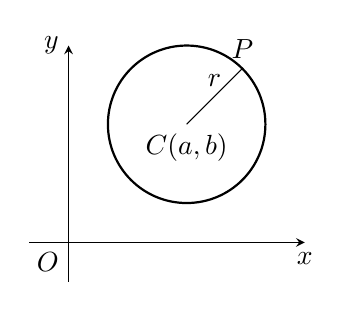
\begin{tikzpicture}[>=stealth]
\draw[->](-.5,0)--(3,0)node[below]{$x$};
\draw[->](0,-.5)--(0,2.5)node[left]{$y$};
\node[below left]{$O$};
\draw[thick](1.5,1.5) circle(1);
\draw(1.5,1.5)node[below]{$C(a,b)$}--node[above]{$r$}+(45:1)node[above]{$P$};



\end{tikzpicture}
\captionof{figure}{}
\end{minipage}



\begin{enumerate}
    \item 设圆心的坐标为$C(a,b)$，圆周上的任意一点为$P(x,y)$.
    \item 点$P$的特征性质是$|CP|=r$\hfill  (*)
    \item 把(*)转化成代数形式，就是$\sqrt{(x-a)^2+(y-b)^2}=r$
\item 化简，得
\begin{equation}
     (x-a)^2+(y-b)^2=r^2 \tag{1}
\end{equation}

\begin{proof}
    由上面求方程的过程可知，圆上点的坐标满足方程(1). 又因为方程化简过程是同解变形，所以坐标满足(1)的点到$C$的距离为$r$，此点在圆上.
\end{proof}
\end{enumerate}

    所以，方程(1)是圆心在$C(a,b)$、半径为$r$的圆的方程. 它称为\textbf{圆的标准方程}.
    
    特别，当圆心在原点时，$a=0$, $b=0$，由(1)可得
\begin{equation}
     x^2+y^2=r^2 \tag{2}
\end{equation}   
    以下我们探求圆方程的一般式.

    把方程(1)写成：$x^2+y^2-2ax-2by+a^2+b^2-r^2=0$. 可见，圆的方程具有形式：
    \begin{equation}
       x^2+y^2+Dx+Ey+F=0    \tag{3}
    \end{equation}
反过来，形如(3)的方程是否都表示圆呢？先看下面的实例.

\begin{example}
下列二元二次方程中哪个表示圆？如是圆，求出其圆心和半径：
\begin{multicols}{2}
\begin{enumerate}[(1)]
    \item $4x^2+4y^2-12x+16y+9=0$
    \item $3x^2+3y^2+12x-24y+60=0$
    \item $x^2+y^2-2x-4y+6=0$
\end{enumerate}    
\end{multicols}
\end{example}

\begin{solution}
\begin{enumerate}[(1)]
    \item \[\begin{split}
        4x^2+4y^2-12x+16y+9&=0\\
x^2+y^2-3x+4y+\frac{9}{4}&=0\\
x^2-3x+\left(\frac{3}{2}\right)^2+y^2+4y+2^2&=-\frac{9}{4}+\frac{9}{4}+4\\
\left(x-\frac{3}{2}\right)^2+(y+2)^2=2^2
    \end{split}\]
$\therefore\quad $此方程表示圆，圆心是$\left(\frac{3}{2},\; -2\right)$，半径$r=2$.

\item \[\begin{split}
    3x^2+3y^2+12x-24y+60&=0\\
    x^2+y^2+4x-8y+20&=0\\
    x^2+4x+2^2+y^2-8y+4^2&=-20+4+16\\
    (x+2)^2+(y-4)^2=0
\end{split}\]
$\therefore\quad $此方程表示一个点$(-2,4)$，不表示圆.

\item \[\begin{split}
    x^2+y^2-2x-4y+6&=0\\
    x^2-2x+1^2+y^2-4y+2^2&=-6+1+4\\
    (x-1)^2+(y-2)^2&=-1
\end{split}\]
$\because\quad $左$\ge 0$，右$=-1$，方程(3)无实数解，即在坐标平面上无轨迹.

$\therefore\quad $此方程不表示任何图形.
\end{enumerate}
\end{solution}

可见，方程(3)有时表示圆，有时仅表示一个点，有时不表示任何图形. 现在探讨方程(3)属于上述几种可能时的条件. 把(3)配方：
\[x^2+Dx+\left(\frac{D}{2}\right)^2+y^2+Ey+\left(\frac{E}{2}\right)^2=-F+\frac{D^2}{4}+\frac{E^2}{4}\]
得
\[\left(x+\frac{D}{2}\right)^2+\left(y+\frac{E}{2}\right)^2=\frac{D^2+E^2-4F}{4}\]
\begin{enumerate}[(i)]
    \item 当$D^2+E^2-4F>0$时，方程(3)表示以$\left(\frac{-D}{2},\; \frac{-E}{2}\right)$为圆心，以$\sqrt{\frac{D^2+E^2-4F}{4}}$为半径的圆；
    \item 当$D^2+E^2-4F=0$时，方程(3)有且仅有一个实数解$x=-\frac{D}{2},\; y=-\frac{E}{2}$，所以只表示一个点$\left(-\frac{D}{2},\; -\frac{E}{2}\right)$
    \item 当$D^2+E^2-4F<0$时，方程(3)没有实数解，因而在坐标平面上不表示任何图形.
\end{enumerate}

综合上述，方程(3)当且仅当$D^2+E^2-4F>0$时，表示圆；方程(3)或更一般的
\[Ax^2+Ay^2+Dx+Ey+F=0\quad (A\ne 0,\; D^2+E^2-4AF>0)\]
称为圆方程的\textbf{一般式}.

注意，上述论证中用的是“\textbf{配方法}”. 这里的书写格式将使我们少出错误，应该熟练掌握.

\subsection*{3.1 练习}
\begin{enumerate}
    \item 写出圆心在$(-4,3)$、半径为5的圆的方程，并检验$A(-1,-1)$、$B(1,2)$、$C(0,0)$、$D(-2,1)$各点是在这个圆内？圆上？还是圆外？
    \item 下列各方程是否表示圆？若是，求出其圆心和半径：
    \begin{multicols}{2}
\begin{enumerate}[(1)]
    \item $x^2+y^2-2x+2y-2=0$
    \item $x^2+y^2+8x+6y=0$
    \item $7x^2+7y^2-4x-y-4=0$
    \item $x^2+y^2+2x-4y+5=0$
    \item $x^2+y^2-4x+10y+31=0$
\end{enumerate}
    \end{multicols}

    \item 下列方程，各表示什么样的圆（应指出圆心和半径）？
    \begin{multicols}{2}
    \begin{enumerate}[(1)]
        \item $x^2+y^2+2ax=0$
        \item $x^2+y^2+2by=0$
        \item $x^2+y^2+2ax-b^2=0$
\end{enumerate}
    \end{multicols}
\end{enumerate}

\section{圆方程的确定}
欲确定圆的方程
\[(x-a)^2+(y-b)^2=r^2\]
或
\[x^2+y^2+Dx+Ey+F=0\quad (D^2+E^2-4F>0)\]
实质是求出其中的参数$a$、$b$、$r$或$D$、$E$、$F$.

\begin{example}
    据下列条件，求圆的方程：
\begin{enumerate}[(1)]
\item 圆心在$(-3,2)$，与直线$2x+3y-6=0$相切的圆.
\item 过$A(2,2)$、$B(5,3)$、$C(6,0)$三个点的圆．
\end{enumerate}
\end{example}

\begin{solution}
\begin{enumerate}[(1)]
    \item $a=-3$, $b=2$
\[r=\frac{|2(-3)+3\x 2-6|}{\sqrt{2^2+3^2}}=\frac{6}{\sqrt{13}}\]
$\therefore\quad $圆方程是$(x+3)^2+(y-2)^2=\frac{36}{13}$
\item \begin{analyze}
由已知条件不易直接求出圆心坐标和半径，我们用一般式.
\end{analyze}

设过$A$、$B$、$C$的圆方程为
\[x^2+y^2+Dx+Ey+F=0\]
由已知，可得$\begin{cases}
    2^2+2^2+2D+2E+F=0\\
    5^2+3^2+5D+3E+F=0\\
    6^2+6D+F=0
\end{cases}$

即
\[\begin{cases}
    2D+2E+F=-8\\ 5D+3E+F=-34\\ 6D+F=-36
\end{cases}\]
解之，得$D=-8,\quad E=-2,\quad F=12$.

$\therefore\quad $圆方程是$x^2+y^2-8x-2y+12=0$
\end{enumerate}
\end{solution}

\begin{example}
    圆过$P(1,3)$、$Q(-2,-2)$，且圆心在直线$\ell:\; x-y-3=0$
上，求圆的方程，并画出这个圆.
\end{example}

\begin{analyze}
 画出草图（3.3）条件涉及圆心，用方程(1)处理.
\end{analyze}

\noindent
\begin{minipage}{.55\textwidth}\CTEXindent
\begin{solution}
设圆心为$C(a,b)$, 利用$|CP|=|CQ|$和$C$在$\ell$上可得
\[\begin{cases}
    \sqrt{(a-1)^2+(b-3)^2}=\sqrt{(a+2)^2+(b-2)^2}\\
    a-b-3=0
\end{cases}\]
解之，得$a=1,\quad b=-2$,
\[r=|CP|=\sqrt{(1-1)^2+(-2-3)^2}=5\]
$\therefore \quad $圆方程为$(x-1)^2+(y+2)^2=25$.

以$(1,-2)$为圆心，以$r=5$为半径的圆为所求（图3.3）．
\end{solution}
\end{minipage}
\hfill
\begin{minipage}{.4\textwidth}
\centering
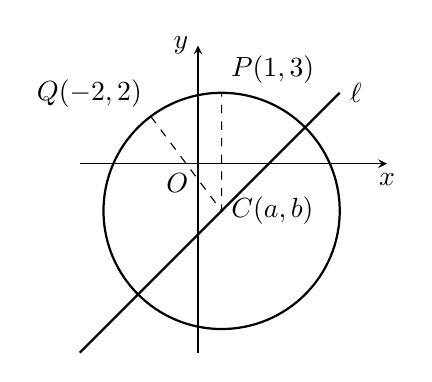
\begin{tikzpicture}[>=stealth, scale=.3]
\draw[->](-5,0)--(8,0)node[below]{$x$};
\draw[->](0,-8)--(0,5)node[left]{$y$};
\node[below left]{$O$};
\draw[thick](1,-2) circle(5);
\draw[dashed](-2,2)node[above left=-.3]{$Q(-2,2)$}--(1,-2)node[right]{$C(a,b)$}--(1,3)node[above right=-.1]{$P(1,3)$};
\draw[domain=-5:6, thick]plot(\x, \x-3)node[right]{$\ell$};
\end{tikzpicture}
\captionof{figure}{}
\end{minipage}

\subsection*{3.2 练习}
\begin{enumerate}
    \item 根据下列条件，求圆的方程：
\begin{enumerate}[(1)]
\item 圆心在点$(2,-4)$，并与直线$x-y=2$相切；
\item 与直线$x=6$, $x=10$都相切，并且过点$(8,3)$；
\item 与$x-2y=0$和$x-2y-6=0$都相切，并且过点$\left(2,\frac{2}{\sqrt{5}}\right)$；
\item 经过点$A(-1,1)$和$B(1,3)$，圆心在$x$轴上；
\item 经过点$A(-4,4)$和$B(2,0)$，并且和直线$2x+3y-17=0$相切；
\item 经过$A(0,,0)$、$B(6,-8)$、$C(10,0)$三个点；
\item 和直线$4x+3y-70=0$相切于点$P(10,10)$，半径是10；
\item 经过点$P(2,-1)$，圆心在直线$\ell_1:\; y+2x=0$上，并且与直线$\ell_2:\; x-y-1=0$相切.   
\end{enumerate}

\item  已知$A(x_1,y_1)$、$B(x_2,y_2)$，
证明：以$AB$为直径的圆的方程是$$(x-x_1)(x-x_2)+(y-y_1)(y-y_2)=0$$
\end{enumerate}

\section{圆与直线的位置关系}
已知圆和直线的方程分别为
\[C:\; (x-a)^2+(y-b)^2=r^2\quad \text{和}\quad \ell:\; Ax+By+D=0\]
它们的位置关系显然有三种情况，可以用圆心到直线的距离$d_{C-\ell}$讨论之：
\begin{itemize}
    \item $C$与$\ell$相离$\Longleftrightarrow d_{C-\ell}>r$
    \item $C$与$\ell$相切$\Longleftrightarrow d_{C-\ell}=r$
    \item $C$与$\ell$相割$\Longleftrightarrow d_{C-\ell}<r$
\end{itemize}
也可以用圆和直线$\ell$的公共点个数讨论之：

它们的公共点坐标由方程组
\begin{equation}
    \begin{cases}
        (x-a)^2+(y-b)^2=r^2\\
        Ax+By+D=0
    \end{cases}\tag{*}
\end{equation}
确定，因此：
\begin{itemize}
    \item $C$与$\ell$相离$\Longleftrightarrow$没有公共点$\Longleftrightarrow$方程组(*)没有实数解；
    \item $C$与$\ell$相切$\Longleftrightarrow$有一个公共点$\Longleftrightarrow$方程组(*)有相同两实数解；
    \item  $C$与$\ell$相割$\Longleftrightarrow$有两个公共点$\Longleftrightarrow$方程组(*)有相异两实数解.
\end{itemize}

而方程组(*)的解的情况，可通过“消元”得到一元二次方程，然后用判别式$\Delta$来讨论.











\begin{example}
    当k取何值时，直线$x+y=k$与圆$x^2+y^2=1$相割、相切、相离？
\end{example}

\begin{solution}
圆$x^2+y^2=1$的圆心$C(0,0)$到直线$x+y-k=0$的距离
\[d=\frac{|x+y-k|}{\sqrt{1^2+1^2}}=\frac{|-k|}{\sqrt{2}},\qquad r=1\]
\begin{enumerate}[(i)]
\item 当$d<r$，即$\frac{|k|}{\sqrt{2}}<1$，也就是$-\sqrt{2}<k<\sqrt{2}$时，直线与圆相割；
\item 当$d=r$，即$k=\pm \sqrt{2}$时，直线与圆相切；
\item 当$d>r$，即$|k|>\sqrt{2}$，也就是$k<-\sqrt{2}$或$k>\sqrt{2}$时，直线与圆相离.
\end{enumerate}
\end{solution}


\begin{example}
    求与直线$\ell_0:\; x+3y=10$相垂直的圆$x^2+y^2=4$的切线的方程.
\end{example}

\begin{solution}
\textbf{解法1：}与$\ell_0$垂直的直线系$\ell$的方程是
\[3x-y+m=0\]
欲使$\ell$成为圆的切线
\[d=\frac{|3x-y+m|}{\sqrt{3^2+(-1)^2}}=\frac{|m|}{\sqrt{10}}=2\]
可得，$m=\pm 2\sqrt{10}$

$\therefore\quad $切线方程是$3x-y\pm 2\sqrt{10}=0$.

\textbf{解法2：}$\ell$与$x^2+y^2=4$的交点坐标满足
\[\begin{cases}
    3x-y+m=0\\ x^2+y^2=4
\end{cases}\]
消去$y$，整理为：$10x^2+6mx+m^2-4=0$
\[\text{$\ell$是圆的切线}\Longleftrightarrow \Delta =(6m)^2-4\cdot 10\cdot (m^2-4)=0\]
即
\[-m^2+40=0\Longleftrightarrow m=\pm2\sqrt{10}\]
$\therefore\quad $切线方程是$3x-y\pm 2\sqrt{10}=0$.
\end{solution}



\begin{example}
已知圆的方程是$x^2+y^2=r^2$. 求证：经过圆上一点$P_0(x_0,y_0)$的切线方程是$x_0x+y_0y=r^2$.
\end{example}

\begin{analyze}
     切线$\ell$过切点$P_0(x_0,y_0)$，所以，只要设法求出斜率$k_{\ell}$即可（图3.4）．
\end{analyze}

\begin{solution}
\begin{enumerate}[(i)]
    \item 当$y_0\ne 0$时，$k_1=-\frac{x_0}{y_0}$,
    
\noindent
\begin{minipage}{.56\textwidth}
$\therefore\quad \ell$的方程是
   \[ y-y_0=-\frac{x_0}{y_0}(x-x_0)\]
    即
\[    y_0y-y+x_0x-x^2_0=0\]
    但是$x^2+y^2=r^2$,  两式相加，得
\begin{equation}
     x_0x+y_0y=r^2 \tag{1}
\end{equation}
    
\end{minipage}
\hfill
\begin{minipage}{.4\textwidth}
\centering
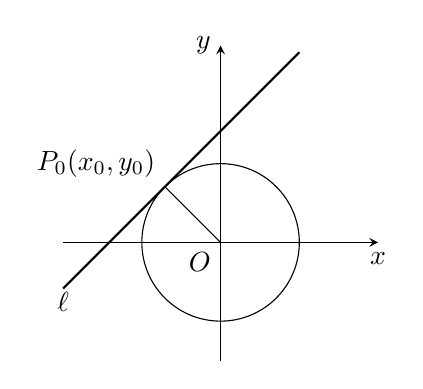
\begin{tikzpicture}[>=stealth]
\draw[->](-2,0)--(2,0)node[below]{$x$};
\draw[->](0,-1.5)--(0,2.5)node[left]{$y$};
\node[below left]{$O$};
\draw(0,0)circle (1);
\draw(0,0)--(45+90:1)node[above left]{$P_0(x_0,y_0)$};
\draw[domain=-2:1, thick]plot(\x, \x+1.414);
\node at (-2,-.75){$\ell$};
\tkzDefPoints{0/0/O, -0.707/.707/P, -1.414/0/A}
\tkzMarkRightAngles[size=.15](O,P,A)
\end{tikzpicture}
\captionof{figure}{}
\end{minipage}
\item 当$y_0=0$时，切线$\ell$垂直$x$轴，方程为
 \[   x=x_0\]
    它仍然可以写成(1)的形式.
\end{enumerate}
    所以，不论（i）或（ii），切线$\ell$的方程都可写成(1).
\end{solution}



\begin{example}
    求经过点$P(6,-4)$且被圆$x^2+y^2=20$截得的弦
长为$6\sqrt{2}$的直线的方程.
\end{example}

\begin{analyze}
    设$\ell_1$为所求($|P_1P_2|=6\sqrt{2}$).

\noindent
\begin{minipage}{.52\textwidth}\CTEXindent
$\because\quad    x^2+y^2=20$是定圆，弦长为定值，

$\therefore\quad $弦心距$|OD|$也是定值：
\[\begin{split}
    |OD|&=\sqrt{|OP_2|^2-|DP_2|^2}\\
    &=\sqrt{20-\left(3\sqrt{2}\right)^2}=\sqrt{2}
\end{split}\]
从而，所求直线$\ell$就是过$P(6,-4)$向圆
$x^2+y^2=2$
所作的两条切线，或者直线$\ell$是过$P(6,-4)$且到原点的距离$d_{\ell-0}=\sqrt{2}$的直线（图3.5）．

以下解的过程留给读者.
\end{minipage}
\hfill
\begin{minipage}{.45\textwidth}
\centering
\begin{tikzpicture}[>=stealth, scale=.3]
\draw[->](-9,0)--(10,0)node[below]{$x$};
\draw[->](0,-8)--(0,8)node[left]{$y$};
\node[above left]{$O$};
\draw[thick](0,0)circle (4.472);
\tkzDefPoints{6/-4/P, 0/0/O, 0/4.472/A, 2/0/A1, -3.714/0/A2}
\draw[domain=7:-4, thick]plot(\x, 2-\x)node[above]{$\ell_1$};
\draw[domain=7:-7, thick]plot(\x, {(-26-7*\x)/17})node[above]{$\ell_2$};
\tkzInterLC(A1,P)(O,A) \tkzGetPoints{P_1}{P_2}
\tkzInterLC(A2,P)(O,A) \tkzGetPoints{B3}{B4}
\node at (P) [right]{$P(6,-4)$};
\tkzDefPointBy[projection = onto A1--P](O) \tkzGetPoint{D}
\tkzLabelPoints[above](P_1,D)
\tkzLabelPoints[right](P_2)
\draw[dashed](P_2)--(O)--(D);
\tkzMarkRightAngles[size=.4](O,D,P_2)
\end{tikzpicture}
\captionof{figure}{}
\end{minipage}

（答：$x+y-2=0$和$7x+17y+26=0$）
\end{analyze}

\begin{remark}
 在这个例题中，圆的半径和弦长都一定，据平面几何知识我们知道弦心距$|OD|$必为定值. 这一点是解决本题的关键.
\end{remark}


\subsection*{3.3 练习}
\begin{enumerate}
    \item 求直线$y=-2x+10$和圆$x^2+y^2=25$的交点坐标，并画图.
    \item 当$b$为何值时，直线$y=2x+b$与圆$x^2+y^2=9$相割、相切、相离.
    \item 证明直线$2x+3y-17=0$与圆$x^2+y^2+2x-4y-8=0$相切.
\end{enumerate}

\section*{习题一}
\begin{center}
    \bfseries A
\end{center}

\begin{enumerate}
    \item 证明下面两图相外切，并画出图形：
    \[x^2+y^2-4x-6y+9=0\quad \text{与}\quad x^2+y^2+12x+6y-19=0\]
\item \begin{enumerate}[(1)]
    \item 求圆$x^2+y^2=25$和圆$x^2+y^2-26y+25=0$的交点，并证明交点连线与两圆圆心连线互相垂直；
    \item 利用2.9节引理求过（1）中两圆两个交点的直线．
\end{enumerate}   
    \item 圆与$x$轴交于两个点$A(a,0)$、$B(b,0)$，其中$ab\ge 0$，并与$y$轴相切，求圆的一般式方程.
    \item 设圆的方程是$x^2+y^2-2ax-2by+c=0$，与两坐标轴相交，求证：
\begin{enumerate}[(1)]
\item 在$x$轴上两截距的和是$2a$，乘积是$c$；
\item 在$x$轴上两截距的差是$\pm 2\sqrt{a^2-c}$;
\item 在$y$轴上两截距的和是$2b$，乘积是$c$；
\item 截两坐标轴所成弦的弦长平方差是$\pm 4(a^2-b^2)$.
\end{enumerate}

\end{enumerate}

\begin{center}
    \bfseries B
\end{center}

\begin{enumerate}\setcounter{enumi}{4}
    \item 求圆$x^2+y^2-2ax\cos\alpha-a^2\sin^2\alpha=0$在$x$轴上截得的弦长.
    \item \begin{enumerate}[(1)]
        \item 过点$P(-2,3)$作圆$x^2+y^2=4$的切线$\ell$，求$\ell$的方程。
        \item 过点$P(-2,3)$作圆$x^2+y^2=4$的两条切线，求同时过两个切点的直线$\ell'$.
    \end{enumerate}  
    \item 求过原点并与直线$x=1$及圆$(x-1)^2+(y-2)^2=1$都相
    切的圆的方程.
    \item 求证：圆$x^2+y^2=r^2$的斜率为$k$的切线方程是$y=kx\pm r\sqrt{1+k^2}$.
    \item 求与直线$2x-y+1=0$垂直的圆$x^2+y^2+5x=0$的切线方程.
    \item 直线$\ell$过点$A(6,17)$，且被圆$x^2+y^2=25$截得的弦长为$4\sqrt{5}$，求$\ell$的方程.
    \item 已知两圆$C_1:\; x^2+y^2-6y=0,\quad C_2:\; (x-2\sqrt{3})^2+(y-1)^2=1$
\begin{enumerate}[(1)]
    \item 求证$C_1$、$C_2$相外切，且$x$轴是它的一条外公切线；
    \item 求切点间的两弧与$x$轴所围成的图形的面积．
\end{enumerate}
  
\end{enumerate}


\section*{二、曲线的参数方程}
\section{曲线的参数方程}
在“曲线与方程”一节中，我们已经看到了曲线$C$与它的方程$F(x,y)=0$之间的对应关系. 认识到$F(x,y)=0$实际上是曲线$C$的代数形式，借助于它实现了用代数方法研究曲线$C$的几何性质的设想.

现在我们引入曲线$C$的另一种代数形式——参数方程，它是用代数方法研究曲线的又一有力工具.

先看一个实例：
炮弹的发射角为$\alpha$，初速度为$v_0$，求弹道曲线的方程（假定不计空气阻力）。

\noindent
\begin{minipage}{.55\textwidth}\CTEXindent
我们以炮口为原点，水平方向为$x$轴，建立坐标系（图3.6）．设炮弹运行曲线上的动点为$P(x,y)$. 可以看出，\textbf{点$P$运动的特征性质不明显，难以找到$x$，$y$之间的直接关系}. 但是，一个非常明显的事实是：点$P$的位置，也就是$(x,y)$由发射后的时
间$t$决定. 事实上，炮弹在$Ox$方向是以$v_x=v_0\cos\alpha$作匀速直线运动的；在$Oy$方向是以$v_y=v_0\sin\alpha$作竖直上抛运动. 由物理学知道
\end{minipage}
\hfill
\begin{minipage}{.43\textwidth}
\centering
\begin{tikzpicture}[>=stealth]
\draw[->](-.5,0)--(5,0)node[below]{$x$};
\draw[->](0,-1.5)--(0,3)node[left]{$y$};
\node[below left]{$O$};
\draw[domain=0:4, thick, smooth, samples=100]plot(\x,{1-0.25*(\x-2)^2});
\draw[dashed](1,0)node[below]{$v_x$}--(1,1)node[above]{$v_0$}--(0,1)node[left]{$v_y$};
\draw[thick, ->](0,0)--(1,1);
\draw(.3,0) arc (0:45:.3)node[right]{$\alpha$};
\node at (2.5,1.25){$P(x,y)$};
\end{tikzpicture}
\captionof{figure}{}
\end{minipage}

\begin{equation}
\begin{cases}
    x=v_x t=v_0\cos\alpha \cdot t\\
    y=v_y t-\frac{1}{2}gt^2= v_0\sin\alpha\cdot t-\frac{1}{2}gt^2
\end{cases} t\ge 0  \tag{1}
\end{equation}
这里，$v_0$，$\alpha$是常数，$g$是重力加速度（取9.8米/秒$^2$）．当$t$取某个允许值时，由方程组(1)就可以确定此刻炮道的确切位置. 这样建立$x$、$y$与辅助变量$t$的关系，不仅十分自然、方便，而且还具有实际意义. 如方程组(1)中的两个方程就分别反映炮弹飞行的水平距离、高度与时间的关系. 这样得到的方程组(1)实际上已经表示出了炮弹运行的弹道曲线.

由此，可以抽象出如下定义.

\begin{thm}
{定义} 在$xOy$坐标系中，若曲线$C$上的任一点的坐标$x$、$y$都能通过第三变量$t$表示出来（纯粹性）：
\begin{equation}
    \begin{cases}
        x=f(t)\\y=\varphi(t) 
    \end{cases}\quad t\in M \tag{2}
\end{equation}
这里$M$是某个指定的区间.反之，对于每个$t\in M$，由(2)确定的点$(x,y)$都在曲线$C$上（完备性）.那么，方程组(2)就叫
做曲线$C$的\textbf{参数方程}. 在(2)中联系$x$、$y$之间关系的辅助变量$t$叫做\textbf{参变数}（简称\textbf{参数}），它可以有物理的或几何的意义，也可以是抽象的变数.
\end{thm}

为了和参数方程相区别，曲线$C$的方程$F(x,y)=0$叫做\textbf{曲线的普通方程}（应注意：普通方程反映的是曲线上的点坐标$x$、$y$之间的直接关系，而在参数方程中$x$、$y$是通过参数$t$间接联系着的）.

\begin{example}
    已知曲线$\ell:\; \begin{cases}
        x=2t\\ y=3t^2+1
    \end{cases}$（t为参数）
\begin{enumerate}[(1)]
\item 判断点$P_1(1,2)$、$P_2(0,1)$与曲线$\ell$的位置关系；
\item 已知点$Q(2,a)$在曲线$\ell$上，求$a$的值.    
\end{enumerate}
\end{example}




\begin{solution}
\begin{enumerate}[(1)]
    \item 把点$P_1$的坐标代入曲线方程，得
\[\begin{cases}
    1=2t\\ 2=3t^2+1
\end{cases}\Rightarrow \begin{cases}
    t=\frac{1}{2}\\[1.5ex]
    t=\pm\frac{\sqrt{3}}{3}
\end{cases}\]
立即得到关于$t$的方程组无解，也就是说点$P$的坐标不能通过参数$t$表示出来，所以点$P$不在曲线$\ell$上.

把点$P_2$的坐标代入曲线方程，解得$t=0$，所以点$P_2$在曲线$\ell$上.

\item $\because\quad Q\in\ell,\qquad \therefore\quad \begin{cases}
    2=2t\\
    a=3t^2+1
\end{cases}$

解得$t=1,\quad a=4$.
\end{enumerate}
\end{solution}

曲线的普通方程和参数方程既然同是曲线的不同的代数形式，它们都是表示曲线上点的坐标之间关系的，从本质上讲它们是相互联系的. 一般情况下可以互化：
\[\text{曲线的参数方程}\xrightleftharpoons[\text{引入参数}]{\text{消去参数}}\text{曲线的普通方程}\]

\begin{example}
    把弹道曲线的参数方程
\[\begin{cases}
    x=v_0t\cos\alpha &   (1)\\
    y=v_0t\sin\alpha-\frac{1}{2}gt^2 &   (2)
\end{cases}\]
化为普通方程，并求出炮弹水平射程的公式.
\end{example}

\begin{solution}
由(1)得：$t=\frac{x}{v_0\cos\alpha}$，
代入(2)，消去参数$t$，得普通方程
\[y=-\frac{g}{2v^2_0\cos^2\alpha}x^2+\frac{\sin\alpha}{\cos\alpha}x\]
这是抛物线方程.

在这个方程里，令$y=0$，得$x_1=0$, $x_2=\frac{v^2_0 \sin2\alpha}{g}$. 炮弹的水平射程公式为
\[s=x_2-x_1=\frac{v^2_0 \sin2\alpha}{g}\]
\end{solution}

\begin{example}
    把参数方程
$\begin{cases}
    x=a\cos\varphi\\ y=b\sin\varphi
\end{cases}(a>b>0)$
化为普通方程.
\end{example}

\begin{solution}
分别将两方程变形得
\[\begin{cases}
    \frac{x}{a}=\cos\varphi\\[1.5ex]
    \frac{y}{b}=\sin\varphi\\
\end{cases}\]
再将两方程的两边平方后相加，得
\[\frac{x^2}{a^2}+\frac{y^2}{b^2}=\cos^2\varphi+\sin^2\varphi\]
即
\[\frac{x^2}{a^2}+\frac{y^2}{b^2}=1\]
这就是所求的普通方程.
\end{solution}



\begin{example}
    设$x=\frac{t}{\sqrt{5}}-\frac{1}{2}\; (t\in\R)$，把直线方程$2x-y+1=0$化成参数方程．
\end{example}

\begin{solution}
把$x=\frac{t}{\sqrt{5}}-\frac{1}{2}$代入方程$2x-y+1=0$，得
\[y=\frac{2t}{\sqrt{5}}\]

$\therefore\quad $直线的参数方程是$\begin{cases}
    x=\frac{t}{\sqrt{5}}-\frac{1}{2}\\[1.5ex]
    y=\frac{2t}{\sqrt{5}}
\end{cases}$
\end{solution}


\begin{remark}
    对于同一曲线，由于参数选择的不同，可有不同形式的参数方程．例3.11中，设$x=t$，则得到直线的另一种形式的参数方程.
    
    在互化时必须使坐标$x$、$y$的取值范围在互化前后保持不变. 否则互化就破坏了轨迹的纯粹性或完备性，就是不等
价的.
\end{remark}

\begin{example}
   曲线$C$的普通方程是$y=x^2$，那么，$\begin{cases}
       x=t^2\\y=t^4
   \end{cases}(t\in\R)$是曲线$C$的参数方程吗？
\end{example}

\begin{solution}
很明显，$y=x^2$与$\begin{cases}
    x=t^2\\y=t^4
\end{cases}(t\in\R)$是不等价的. 事实上，在$y=x^2$中，$x\in\R$；而在$\begin{cases}
    x=t^2\\y=t^4
\end{cases}(t\in\R)$中$x\ge 0$. 所以，后者不是曲线$C$的参数方程.

$y=x^2$与$\begin{cases}
    x=t^2\\y=t^4
\end{cases}(t\in\R)$是等价的，所以，$\begin{cases}
    x=t^2\\y=t^4
\end{cases}(t\in\R)$是曲线$C$的一种参数方程.

引入曲线的参数方程，对解决一些问题提供了简便的方法.
\end{solution}

\begin{example}
    已知直线$\ell_1:\; x-ky+k=0,\quad \ell_2:\; kx-y-1=0$，其中$k$为参数，求$\ell_1,\ell_2$的交点的轨迹方程.
\end{example}

\begin{analyze}
    常想到的办法是求交点.如果从曲线与方程的概念出发，设交点为$P(x,y)$，它的坐标满足方程$x-ky+k=0$和$kx-y-1=0$，因此也就满足由这两个方程得到的同解方程. 于是就有两种解法.
\end{analyze}

\begin{solution}
\textbf{解法1：}解方程组
\[\begin{cases}
    x-ky+k=0\\ kx-y-1=0
\end{cases}\]
当$k^2\ne 1$时，得到$$\begin{cases}
    x=\frac{2k}{k^2-1}\\[1.5ex]
    y=\frac{k^2+1}{k^2-1}\\
\end{cases}\text{（$k$是参数）}$$
这便是所求轨迹的参数方程. 但如果要求轨迹的普通方程，需要消去参数k，那将是比较复杂的.

\textbf{解法2：}由$kx-y-1=0$，当$x\ne 0$时，可得$k=\frac{y+1}{x}$，代入方程$x-ky+k=0$，得
\[x-\frac{y^2+y}{x}+\frac{y+1}{x}=0\]
去分母，化简得
\[x^2-y^2+1=0,\quad (x\ne 0)\]

$x=0$时，存在$k=0$，使得$y=-1$. 于是，我们得到所求轨迹的普通方程为$x^2-y^2+1=0,\quad (y\ne 1)$.
\end{solution}

\begin{remark}
     解法2中，方程两边同除以$x$会丢$x=0$的解，方程两边同乘以$x$会增$x=0$的解，所以最后得到轨迹方程后应检验是否是同解变形.

     两种方法得到轨迹的不同形式的方程，只要把参数方程的参数消去，便可得到同样的普通方程，读者不妨试一试.
\end{remark}

\subsection*{3.4 练习}
\begin{enumerate}
    \item 判断下列各题中点与曲线的位置关系：
\begin{enumerate}[(1)]
    \item $P\left(1,3-3\sqrt{3}\right)$与曲线$C:\; \begin{cases}
        x=-2-\frac{1}{2}t\\[1.5ex] y=3+\frac{\sqrt{3}}{2}t
    \end{cases}$
    \item $A\left(\frac{5}{2},\; -\frac{5\sqrt{3}}{2}\right)$与曲线$\ell:\; \begin{cases}
        x=5\cos\theta\\ y=5\sin\theta
    \end{cases}$
    \item $B\left(\frac{1}{2},1\right)$与曲线$C:\; \begin{cases}
        x=\sec\varphi \\ y=\tan\varphi
    \end{cases}$
    \item $C\left(-\frac{1}{2},\; \frac{\sqrt{3}}{2}\right)$与曲线$\ell:\; \begin{cases}
        x=\sin\alpha \\  y=2\cos\alpha
    \end{cases}$
\end{enumerate}

\item 把下列曲线的参数方程（$\alpha$，$t$是参数）化成普通方程：
\begin{multicols}{2}
\begin{enumerate}[(1)]
    \item $\begin{cases}
        x=2\cos\alpha\\
        y=3\sin\alpha
    \end{cases}$
    \item $\begin{cases}
        x=2pt^2\\
        y=2pt
    \end{cases}(p>0)$
    \item $\begin{cases}
        x=x_1+at\\
        y=y_1+bt
    \end{cases}(b\ne 0)$
    \item $\begin{cases}
        x=t-1\\
        y=t^2+2t-8
    \end{cases}$
\end{enumerate}
\end{multicols}
\item 根据所给条件，把下列各方程化成参数方程：
\begin{enumerate}[(1)]
    \item $xy=a^2\; (a\ne 0)$，设$x=a\tan\varphi$，$\varphi$是参数；
    \item $\frac{x^2}{a^2}-\frac{y^2}{b^2}=1$，设$y=b\tan\varphi$，$\varphi$是参数.
\end{enumerate}
\end{enumerate}

\section{直线与圆的参数方程}
\subsection{直线的参数方程}
已知$\ell$是过点$P_0(x_0,y_0)$，且倾角为$\alpha$的直线（图3.7）．现在我们来推求它的参数方程.

\noindent
\begin{minipage}{.52\textwidth}\CTEXindent
    在直线$\ell$上，以向上的方向为正方向，以$P_0$为有向直线的坐标原点，单位长与$xOy$坐标系相同，建立直线坐标系（一维坐标系）.那么$P_0$的一维坐标是0，设点$P$的一维坐标是$t$，
    则有向线段$\overline{P_0P}$的数量$\overline{P_0P}=t$. 这样点$P$的位置由$t$确定. 于是产生了一个新问题：$\ell$上同一个点$P$的两种坐标$(x,y)$与$(t)$之间有什么关系呢？
\end{minipage}
\hfill
\begin{minipage}{.45\textwidth}
\centering
\begin{tikzpicture}[>=stealth]
\draw[->](-1.5,0)--(4,0)node[below]{$x$};
\draw[->](0,-1)--(0,3)node[left]{$y$};
\node[below left]{$O$};
\tkzDefPoints{1/1/P0, 3/2/P, 3/1/Q}
\tkzDrawLines[add=1.3 and .4, very thick](P0,P)
\tkzDrawPoints(Q,P,P0)
\draw[dashed](1,0)node[below]{$x_0$}--(P0)node[above left]{$P_0(x_0,y_0)$}--(Q)node[right]{$Q(x,y_0)$};
\draw[dashed](3,0)node[below]{$x$}--(P)node[above left]{$P(x,y)$};
\draw(-.5,0)arc (0:26.56:.5)node[right]{$\alpha$};
\end{tikzpicture}
\captionof{figure}{}
\end{minipage}

从图3.7容易看出：
\begin{equation}
    \begin{cases}
        x=x_0+t\cos\alpha\\
        y=y_0+t\sin\alpha
    \end{cases}t\in\R  \tag{1}
\end{equation}

这样得到的(1)实际上就是$\ell$的一种参数方程（$t$为参数）. 事实上，任取$t\in\R$，由(1)确定的$(x,y)$必在$\ell$上；反之，对于$\ell$上任一点，由于它的一维坐标是确定的，其坐标$x$，$y$总能写成(1)的形式.

由于始点$P_0(x_0,y_0)$和倾角$\alpha$是已知的，因此(1)称为$\ell$的\textbf{点角式参数方程}.

\begin{example}
写出过点$A(1,-2)$，倾角为$45^{\circ}$的直线的点角式参数方程. 若$\ell_1$与$\ell_2:\; x+2y-4=0$相交于$B$（图3.8):
\begin{multicols}{2}
    \begin{enumerate}[(1)]
        \item 求$|AB|$.
        \item 求点$B$的坐标．
    \end{enumerate}
\end{multicols}
\end{example}

\begin{solution}
    $A(1,-2)$为始点，倾角为$45^{\circ}$的直线的点角式参数方程为
\begin{equation}
    \begin{cases}
        x=1+t\cos45^{\circ} \\ y=-2+t\sin 45^{\circ}
    \end{cases}\Rightarrow \begin{cases}
        x=1+\frac{\sqrt{2}}{2}t\\[1.5ex]
        y=-2+\frac{\sqrt{2}}{2}t
    \end{cases}t\in\R \tag{*}
\end{equation}
\begin{enumerate}[(1)]
\noindent
\begin{minipage}{.45\textwidth}
\item 欲计算$|AB|$，可以先算出点$B$相对于点$A$的直线坐标$t$，为此，把(*)代入$\ell_2$的方程，得
\[\left(1+\frac{\sqrt{2}}{2}t\right)+2\left(-2+\frac{\sqrt{2}}{2}t\right)-4=0\]
解出$t=\frac{7}{3}\sqrt{2}$\hfill (**)

$\therefore\quad |AB|=|0-t|=\frac{7}{3}\sqrt{2}$.
\end{minipage}
\hfill
\begin{minipage}{.5\textwidth}
\centering
\begin{tikzpicture}[>=stealth, scale=.6]
\draw[->](-2,0)--(7,0)node[below]{$x$};
\draw[->](0,-4)--(0,3.5)node[left]{$y$};
\node[below left]{$O$};
\tkzDefPoints{1/-2/A, 2/-1/A1, 1/1.5/C, 3/.5/C1}
\tkzDrawLines[add=2 and 3](A,A1)
\tkzDrawLines[add=1 and 1.5](C,C1)
\tkzInterLL(A,A1)(C,C1) \tkzGetPoint{B}
\tkzLabelPoints[above](B)
\tkzDrawPoints(A)
\node at (A)[below right]{$A(1,-2)$};
\node at (-1,3){$\ell_2$};
\node at (5.5,2){$\ell_1$};


\end{tikzpicture}
\captionof{figure}{}
\end{minipage}


    
\item 把(**)代入(*)，得
\[\begin{cases}
    x=1+\frac{\sqrt{2}}{2}\cdot\frac{7\sqrt{2}}{3}=\frac{10}{3}\\[1.5ex]
    y=-2+\frac{\sqrt{2}}{2}\cdot \frac{7\sqrt{2}}{3}=\frac{1}{3}
\end{cases}\Rightarrow B\left(\frac{10}{3},\; \frac{1}{3}\right)\]
\end{enumerate}
\end{solution}

\begin{remark}
    此例使我们初步看到：使用点角式参数方程求距离$|AB|$是多么简捷！
\end{remark}



\begin{example}
圆$x^2+y^2=8$内有一点$P_0(-1,2)$, $AB$为过$P_0$且倾角为$\alpha$的弦.
\begin{enumerate}[(1)]
\item 当$\alpha=\frac{3\pi}{4}$时，求$|AB|$;
\item 当弦$A'B'$被点$P_0$平分时，写出直线$A'B'$的方程.   
\end{enumerate}
\end{example} 

\begin{analyze}
    这是过定点$P_0$的有关弦长的计算问题，因而可用直线的点角式参数方程解.
\end{analyze}

\begin{solution}
设直线$AB$的方程为
\begin{equation}
\begin{cases}
    x=-1+t\cos\alpha\\ y=2+t\sin\alpha  
\end{cases}\tag{1}
\end{equation}
把(1)代入$x^2+y^2=8$，整理得
\begin{equation}
  t-2(\cos\alpha-2\sin\alpha)t-3=0 \tag{2}  
\end{equation}

$\because \quad $直线与圆相交，$\qquad \therefore\quad $(2)有实根.

设$t_1,t_2$是(2)的两个实根，则由韦达定理得
\begin{equation}
 t_1+t_2=2(\cos\alpha-2\sin\alpha),\qquad t_1\cdot t_2=-3 \tag{3}   
\end{equation}

\begin{enumerate}[(1)]

\noindent
\begin{minipage}{.55\textwidth}
 \item 当$\alpha=\frac{3\pi}{4}$（图3.9），
\[\begin{split}
   | AB|^2&=|t_1-t_2|^2=(t_1+t_2)^2-4t_1t_2\\
&=\left[2\left(\cos\frac{3\pi}{4}-2\sin \frac{3\pi}{4}\right)\right]^2-4\x(-3)\\
&=(-3\sqrt{2})^2+12=30
\end{split}\]
$\therefore\quad |AB|=\sqrt{30}$


\end{minipage}
\hfill
\begin{minipage}{.4\textwidth}
\centering
\begin{tikzpicture}[>=stealth, scale=.5]
\draw[->](-4,0)--(4,0)node[below]{$x$};
\draw[->](0,-4)--(0,4)node[left]{$y$};
\node[below left]{$O$};
\draw(0,0)circle (2*1.414);
\tkzDefPoints{0/1/C1, 1/0/C2, 0/0/O, 2.828/0/D, -1/2/P_0}
\tkzInterLC(C1,C2)(O,D) \tkzGetPoints{A}{B}

\tkzDefPoints{-1/2/E1, -3/1/E2}
\tkzInterLC(E1,E2)(O,D) \tkzGetPoints{B'}{A'}
\tkzLabelPoints[above](A,A')
\tkzLabelPoints[right](B)
\tkzLabelPoints[below](P_0)
\tkzLabelPoints[left](B')

\tkzDrawSegments[thick](A,B A',B')
\draw(1.5,0) arc (0:135:.5)node[above right]{$\alpha$};

\end{tikzpicture}
\captionof{figure}{}
\end{minipage}   
\item 弦$A'B'$被点$P_0$平分$\Longleftrightarrow \begin{cases}
    t_1+t_2=0\\ \Delta >0
\end{cases}$

这里$\Delta>0$显然成立. 利用(3)得
\[2(\cos\alpha-2\sin\alpha)=0\quad \Rightarrow\quad  \tan\alpha=\frac{1}{2}=k\]
$\therefore\quad $直线$A'B'$的方程为$y-2=\frac{1}{2}(x+1)$
即
$$x-2y+5=0$$
\end{enumerate}
\end{solution}

\begin{remark}
在（1）中，我们用$|t_1-t_2|$表示$|AB|$；在（2）中，利用弦$A'B'$被点$P_0$平分$\Longleftrightarrow \begin{cases}
    t_1+t_2=0\\ \Delta >0
\end{cases}$这些都具有普遍意义.
\end{remark}

\subsection{圆的参数方程}
\noindent
\begin{minipage}{.5\textwidth}\CTEXindent
    对于$\odot O:\; x^2+y^2=R^2$，根据任意角三角函数的定义有（图3.10）
    \[\begin{cases}
        \frac{x}{R}=\cos\theta\\[1.5ex]
        \frac{y}{R}=\sin\theta
    \end{cases}\theta\in[0,2\pi)\]
    即
    \begin{equation}
    \begin{cases}
        x=R\cos\theta\\
        y=R\sin\theta
    \end{cases}\theta\in[0,2\pi) \tag{1}
    \end{equation}
\end{minipage}
\hfill
\begin{minipage}{.45\textwidth}
\centering
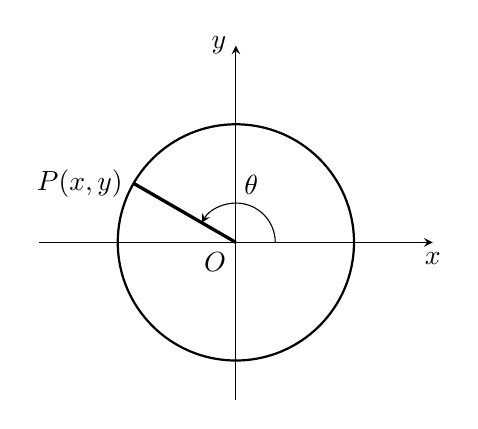
\begin{tikzpicture}[>=stealth]
\draw[->](-2.5,0)--(2.5,0)node[below]{$x$};
\draw[->](0,-2)--(0,2.5)node[left]{$y$};
\node[below left]{$O$};
\draw[thick](0,0)circle(1.5);
\draw[very thick](0,0)--(150:1.5)node[left]{$P(x,y)$};
\draw[->](.5,0) arc (0:150:.5);
\node at (75:.75){$\theta$};

\end{tikzpicture}
\captionof{figure}{}
\end{minipage}

根据曲线参数方程的定义，(1)是$\odot O$的参数方程，其中参数$\theta$有明显的几何意义，它是$Ox$轴正半轴转到射线$OP$所成的角. 为了简单，不妨规定$\theta\in[0,2\pi)$.

\subsection*{3.5 练习}
\begin{enumerate}
    \item 下列各式中，哪一个是直线的点角式参数方程？试述理由. 若是点角式参数方程时，写出始点和倾角.
\begin{multicols}{3}
\begin{enumerate}[(1)]
    \item $\begin{cases}
        x= -2-\frac{1}{2}t  \\[1.5ex]
        y= 3+\frac{\sqrt{3}}{2}t 
    \end{cases}$
    \item $\begin{cases}
        x= 3+2t  \\
        y=  1+3t
    \end{cases}$
    \item $\begin{cases}
        x= -2-\frac{\sqrt{3}}{2}t  \\[1.5ex]
        y= 2-\frac{1}{2}t 
    \end{cases}$
\end{enumerate}
\end{multicols}
    \item 指出下列参数方程表示什么曲线：
\begin{multicols}{2}
\begin{enumerate}[(1)]
    \item $\begin{cases}
        x= 3\cos\varphi  \\
        y=  3\sin\varphi
    \end{cases}\varphi\in\left[0,\frac{\pi}{2}\right]$
    \item $\begin{cases}
        x= \cos\alpha  \\
        y= \sin\alpha 
    \end{cases}\alpha\in (\pi,2\pi)$
    \item $\begin{cases}
        x= 3+5\cos\theta  \\
        y=  2+5\sin\theta
    \end{cases}$
\end{enumerate}
\end{multicols}

\item 求图$\begin{cases}
    x=4+2\cos\varphi\\ 
    y=2+2\sin\varphi
\end{cases}$的圆心坐标和半径的长.
\end{enumerate}

\section*{习题二}
\begin{center}
    \bfseries A
\end{center}

\begin{enumerate}
    \item 已知弹道曲线的参数方程是$\begin{cases}
        x=v_0+\cos\alpha\\
        y=v_0+\sin\alpha-\frac{1}{2}gt^2 
    \end{cases}\text{（ $t>0$,\; $t$是参数）}$
\begin{enumerate}[(1)]
\item 求发射角$\alpha=\frac{\pi}{3}$时，弹道曲线的普通方程和射程.
\item 设$v_0$是定值，$\alpha$可以变动，求证：$\alpha=\frac{\pi}{4}$时射程最大.
\end{enumerate}
\item 把下列参数方程化为普通方程（其中$\varphi$、$t$是参数）：
\begin{multicols}{2}
\begin{enumerate}[(1)]
    \item $\begin{cases}
        x= 3-4\tan\varphi\\
        y=2+3\sec\varphi
    \end{cases}$
    \item $\begin{cases}
        x= \frac{a}{2}\left(
            t+\frac{1}{t}
        \right)\\
        y=\frac{b}{2}\left(t-\frac{1}{t}\right)
    \end{cases}(ab\ne 0)$
\end{enumerate}
\end{multicols}
\item 根据所给条件，化下列方程为参数方程（$t$和$\varphi$是参数）：
\begin{enumerate}[(1)]
    \item $y^2=4x^2-5x^3,\qquad y=tx$;
    \item $4x^2+y^2-16x+12=0,\qquad y=2\sin\varphi$.
\end{enumerate}
\end{enumerate}

\begin{center}
    \bfseries B
\end{center}

\begin{enumerate}\setcounter{enumi}{3}
    \item \begin{enumerate}[(1)]
    \item 写出经过点$M(1,5)$，倾角是$\frac{\pi}{3}$的直线$\ell$的点角式参数方程；
    \item （1）中$\ell$与$\ell':\; x-y-2\sqrt{3}=0$相交于$N$，求$|MN|$和点$N$的坐标；
    \item  若直线$\ell$与圆：$x^2+y^2=16$相交于$P_1,P_2$，求$|MP_1|+|MP_2|$、$|MP_1|\cdot |MP_2|$和$|P_1P_2|$的值.      
    \end{enumerate}
    \item 已知直线$\ell_1:\;x+y=3-\cos4\theta,\quad \ell_2:\; x-y=4\sin2\theta$，求$\ell_1$、$\ell_2$的交点的轨迹方程（$\theta$为参数）.
    \item 已知一条直线上两点$M_1(-1,-1)$、$M_2(1,3)$，以动点$M(x,y)$分$\overline{M_1M_2}$所成的比$\lambda$为参数，写出动点$M$的轨迹的参数方程.
    \item 动点$M$作等速直线运动，它在$x$轴和$y$轴方向的分速度分别为9和12，运动开始时，点位于$A(1,1)$，求点$M$的轨迹的参数方程.
    \item 把下列曲线的参数方程化为普通方程：
\begin{multicols}{2}
\begin{enumerate}[(1)]
    \item $\begin{cases}
        x= t+\frac{1}{t}\\[1.5ex]
        y= t^2+\frac{1}{t^2} 
    \end{cases}$
    \item $\begin{cases}
        x= \sin\alpha\\
        y= \cos2\alpha
    \end{cases}$
\end{enumerate}
\end{multicols}
\end{enumerate}


\section*{三、由曲线的方程画曲线}
\section{由曲线的方程画曲线}
由于直线和圆是最简单的曲线，因此在研究直线和圆的方程时，我们没有讨论由曲线的方程画曲线的问题. 当我们进一步研究较复杂的曲线方程时，就有必要讨论这一问题.

由方程画方程的曲线与由解析式画函数的图象一样，基本方法是\textbf{描点法}. 步骤是：
\begin{enumerate}[(1)]
    \item 列表：在变量取值范围内，给$x$（或$y$）一系列值，求出$y$（或$x$）的对应值，列成表；
    \item 描点：在坐标平面上，以上述$x$、$y$的对应值为坐标，描出一系列对应的点；
    \item 连线：在$x$（或$y$）的取值范围内，把得到的对应点依次用光滑曲线连结起来，这样得到的曲线就是方程的曲线.点取的越多，就越准确.
\end{enumerate}

    如果在用描点法画曲线之前，先对方程进行讨论，以确定曲线的某些几何性质，这不但能较准确、迅速、完整地画出曲线，而且对深入了解曲线的性质也是必要的.这种讨论一般包括以下几点：

    设曲线的方程为$F(x,y)=0$.

\begin{enumerate}
    \item 曲线的范围：
    
    通过讨论方程$F(x,y)=0$中变量$x$、$y$的取值范围，确定曲线存在的范围. 可由$F(x,y)=0$解出$y=f(x)$，求$f(x)$的定义域得到变量$x$的取值范围；由$F(x,y)=0$解出$x=g(y)$，求$g(y)$的定义域得到$y$的取值范围. 也可用不等式估值的方法求$x$、$y$的取值范围.
    \item 曲线关于坐标轴或原点的对称性：
    
    根据关于轴和原点对称的定义容易得到，在$x$、$y$的取值范围内，
\begin{itemize}
    \item   曲线对称于$y$轴$\Longleftrightarrow$ $(x,y)$与$(-x,y)$同时适合方程
    $F(x,y)=0$;
    \item   曲线对称于$x$轴$\Longleftrightarrow$ $(x,y)$与$(x,-y)$同时适合方程
    $F(x,y)=0$;
    \item   曲线对称于原点$\Longleftrightarrow$ $(x,y)$与$(-x,-y)$同时适合方程
    $F(x,y)=0$.
\end{itemize}
  
很容易得到，在上述三种对称中，曲线若具有任何两种对称性质，则一定具有第三种对称性质.
\item 曲线的横、纵截距：

曲线的横截距是指曲线与$x$轴交点的横坐标，纵截距是指曲线与$y$轴交点的纵坐标，它的几何意义分别是从原点到相应交点的有向线段的数量. 根据曲线交点的有关知识，曲线的横截距和纵截距分别由方程组
\[\begin{cases}
    F(x,y)=0\\ y=0
\end{cases}\quad \text{和}\quad \begin{cases}
    F(x,y)=0\\ x=0
\end{cases}\text{确定}\]
\end{enumerate}

以上三方面是研究曲线几何性质的一般要求，对于具体的曲线有时还会讨论其他的性质.

\begin{example}
    画出方程$4x^2+9y^2=36$的曲线.
\end{example}

\begin{solution}
先讨论曲线的几何性质，然后画图.
\begin{enumerate}[(1)]
    \item 范围
    
\textbf{方法1：}由方程$4x^2+9y^2=36$可得
\[\begin{split}
    y=\pm \frac{2}{3}\sqrt{9-x^2},&\qquad |x|\le 3\\
    x=\pm \frac{3}{2}\sqrt{4-y^2},&\qquad |y|\le 2
\end{split}\]
所以曲线位于直线$x=\pm 3$和$y=\pm 2$所围成的矩形里.

\textbf{方法2：}由方程$4x^2+9y^2=36$可得
\[\begin{split}
    4x^2\le 36&\quad \Rightarrow \quad x^2\le 9\quad \Rightarrow \quad |x|\le 3\\
    9y^2\le 36&\quad \Rightarrow \quad y^2\le 4\quad \Rightarrow\quad  |y|\le 2\\
\end{split}\]
所以曲线位于直线$x=\pm 3$和$y=\pm 2$所围成的矩形里.

\item 对称性

在$x$、$y$的取值范围内，$(x,y)$与$(-x,y)$同时适合方程$4x^2+9y^2=36$，所以曲线关于$y$轴对称；$(x,y)$与$(x,-y)$同时适合方程$4x^2+9y^2=36$，所以曲线关于$x$轴对称. 因此，曲线关于原点对称.
\item 截距
\[\begin{split}
    \begin{cases}
        4x^2+9y^2=36\\ y=0
    \end{cases}&\Rightarrow x^2=9\quad \Rightarrow\quad x=\pm3\\
    \begin{cases}
        4x^2+9y^2=36\\ x=0
    \end{cases}&\Rightarrow y^2=4\quad \Rightarrow\quad y=\pm2\\
\end{split}\]
所以曲线的横截距为$\pm 3$，纵截距为$\pm 2$．
\end{enumerate}

现用描点法画图：
\begin{enumerate}[(i)]
    \item 由方程$4x^2+9y^2=36$可得$y=\pm\frac{2}{3}\sqrt{9-x^2}$. 根据曲线的对称性可以先画出曲线在第一象限的图形.为此，根据

\noindent
\begin{minipage}{.45\textwidth}
    \[y=\frac{2}{3}\sqrt{9-x^2}\qquad (0\le x\le 3)\]
    算出几个点的坐标$(x,y)$：    
\begin{center}
\begin{tabular}{c|cccccc}
\hline    
    $x$ &0&1&2&2.5&3&$\cdots$\\
\hline    
$y$&2&1.9&1.5&1.1&0&$\cdots$\\
\hline    
\end{tabular}
\end{center}

\item 描出上述五个对应点，并用光滑曲线连结起来；
\item 利用曲线的对称性画出整个曲线（图3.11）．

\end{minipage}
\hfill
\begin{minipage}{.45\textwidth}
\centering
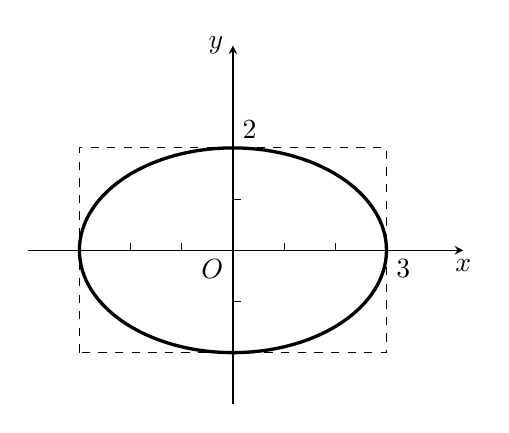
\begin{tikzpicture}[>=stealth, scale=.65]
\draw[->](-4,0)--(4.5,0)node[below]{$x$};
\draw[->](0,-3)--(0,4)node[left]{$y$};
\node[below left]{$O$};
\draw[dashed](-3,-2) rectangle (3,2);
\draw[very thick](0,0)ellipse (3 and 2);
\foreach \x in {1,2}
{
    \draw(\x,0)--(\x,.15);
    \draw(-\x,0)--(-\x,.15);
    \draw(0,\x)--(.15,\x);
    \draw(0,-\x)--(.15,-\x);
}
\node at (0,2)[above right]{2};
\node at (3,0)[below right]{3};

\end{tikzpicture}
\captionof{figure}{}
\end{minipage}
\end{enumerate}
\end{solution}

\begin{example}
画出方程$4x-y^2-8=0$的曲线.
\end{example}

\begin{solution}
讨论：
\begin{enumerate}[(1)]
    \item 范围

    由方程$4x-y^2-8=0$得到$y^2=4x-8$，有
   \[ 4x-8\ge 0 \quad \Rightarrow\quad x\ge 2,\quad y\in\R\]
    所以曲线位于直线$x=2$为边界的右半平面，当$x$的值增大时，$|y|$也增大，这说明曲线向右上方和右下方无限延伸.
    \item 对称性
    
    由于$(x,y)$与$(x,-y)$同时满足方程$4x-y^2-8=0$, 所以曲线关于$x$轴对称.
    \item 截距
\[\begin{cases}
    4x-y^2-8=0\\y=0
\end{cases}\Rightarrow x=2,\qquad \begin{cases}
    4x-y^2-8=0\\x=0
\end{cases}\text{无解}\]    
所以曲线横截距为2，与$y$轴无交点．
\end{enumerate}

    描点法画图：

    \begin{enumerate}[(i)]
\noindent
\begin{minipage}{.48\textwidth}
\item 由方程$4x-y^2-8=0$可得$y=\pm\sqrt{4x-8}$. 根据曲线的对称性先画出曲线在第一象限的图形.为此，根据$y=\sqrt{4x-8}$计算出曲线在第一象限内的$n$个点的坐标，得
    \begin{center}
\begin{tabular}{c|cccccc}
\hline    
    $x$ &2&4&6&8&10&$\cdots$\\
\hline    
$y$&0&2.82&4&4.99&5.64&$\cdots$\\
\hline    
\end{tabular}
\end{center}

\item 描出上述五个对应点，并用光滑曲线连结起来.
\end{minipage}
\hfill
\begin{minipage}{.45\textwidth}
\centering
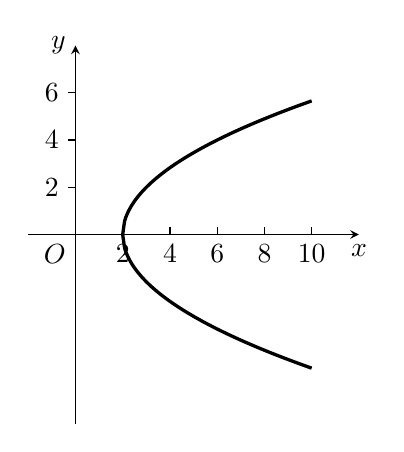
\begin{tikzpicture}[>=stealth, scale=.3]
\draw[->](-2,0)--(12,0)node[below]{$x$};
\draw[->](0,-8)--(0,8)node[left]{$y$};
\node[below left]{$O$};
\draw[domain=2:10, very thick, smooth, samples=100]plot(\x, {sqrt(4*\x-8)});
\draw[domain=2:10, very thick, smooth, samples=100]plot(\x, {-sqrt(4*\x-8)});
\foreach \x in {2,4,6}
{
    \draw(\x, 0)node[below]{\x}--(\x,.3);
    \draw(0,\x)--(-.3,\x)node[left]{\x};
}
\foreach \x in {8,10}
{
    \draw(\x, 0)node[below]{\x}--(\x,.3);
}
\tkzDefPoints{2/0/A, 4/2.82/B, 6/4/C, 8/4.99/D, 10/5.64/E}
\tkzDrawPoints(A,B,C,D,E)
\end{tikzpicture}
\captionof{figure}{}
\end{minipage}

\item 利用曲线的对称性，画出整个曲线（图3.12）．
\end{enumerate}
\end{solution}





由曲线的方程画曲线，有时会遇到一些特殊情况.
\begin{enumerate}
    \item 在曲线$F(x,y)=0$的存在范围$Q$内，若方程$F(x,y)=0$的左边能分解成几个因式的乘积. 那么，在$Q$上使每个因式等于零的方程就对应一条曲线，则这些曲线的全体就是方程$F(x,y)=0$的曲线.
    
    例如方程$(y-\log_2 x)(x^2-y^2)=0$，它的曲线存在范围是
$x>0,\; y\in\R$，即$y$轴的右半平面. 那么由

\noindent
\begin{minipage}{.4\textwidth}

\[\begin{split}
    y-\log_2 x=0 &\quad (x>0)\\
    x-y=0 &\quad (x>0)\\
     x+y=0 &\quad (x>0)\\
\end{split}\]
三个方程所确定的曲线的全体就是方程$(y-\log_2x)(x^2-y^2)=0$的曲线（图3.13），在这类问题中，应该注意曲线存在的范围，否则将导致错误.
\end{minipage}
\hfill
\begin{minipage}{.52\textwidth}
\centering
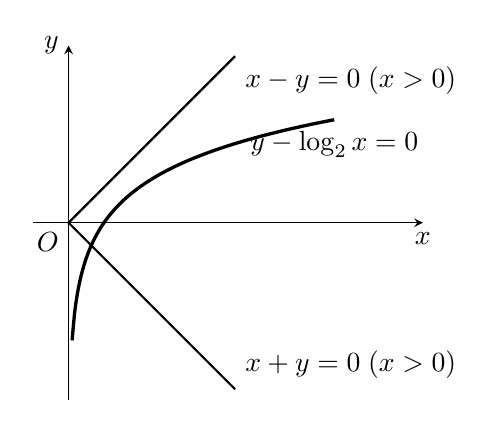
\begin{tikzpicture}[>=stealth, scale=.45]
\draw[->](-1,0)--(10,0)node[below]{$x$};
\draw[->](0,-5)--(0,5)node[left]{$y$};
\node[below left]{$O$};
\draw[thick](4.7,4.7)node[below right]{$x-y=0\; (x>0)$}--(0,0)--(4.7,-4.7)node[above right]{$x+y=0\; (x>0)$};
\draw[domain=.1:7.5, samples=100, very thick, smooth]plot(\x, {ln(\x)/ln(2)})node[below=.2]{$y-\log_2 x=0$};

\end{tikzpicture}
\captionof{figure}{}
\end{minipage}

\item 如果方程只有有限个实数解，那么方程的曲线就是几个点.

例如$x^2+y^2=0$的曲线是原点$(0,0)$. $(x^2-1)^2+(y-4)^2=0$的曲线是两个点$A(1,4)$、$B(-1,4)$.
\end{enumerate}    

\section*{习题三}
\begin{center}
    \bfseries A
\end{center}

\begin{enumerate}
    \item 求下列各曲线的范围：
\begin{multicols}{2}
\begin{enumerate}[(1)]
\item $2x^2+y^2-4x-2y-7=0$
\item $y^2-x^2＝3x+2$
\item $8x+y^2+24=0$
\item $\arctan x=\arctan y$
\end{enumerate}
\end{multicols}

    \item  讨论下列曲线的对称性：
\begin{multicols}{2}
\begin{enumerate}[(1)]
    \item $x^2=8y$
    \item $\frac{x^2}{4}-\frac{y^2}{9}=1$
    \item $x^3+y^3=4xy$
    \item $y-\lg\left(x+\sqrt{x^2+1}\right)=0$
\end{enumerate}    
\end{multicols}


    \item 求下列曲线的截距：
\begin{multicols}{2}
\begin{enumerate}[(1)]
    \item $5x^2-7y^2=35$
    \item $x^2-2xy+y^2+2y-1=0$
\end{enumerate}
\end{multicols}
\end{enumerate}


\begin{center}
    \bfseries B
\end{center}

\begin{enumerate}\setcounter{enumi}{3}
    \item 讨论并画出下列方程的曲线：
\begin{multicols}{3}
    \begin{enumerate}[(1)]
\item $y=x^2-2$
\item $4x^2+y^2=4$
\item $x^2-4y^2=4$
    \end{enumerate}
\end{multicols}

    \item 画出下列方程的曲线：
\begin{multicols}{2}
\begin{enumerate}[(1)]
    \item $x^2-4y^2=0$
    \item $(x+3y-4)(x^2+y^2-4)=0$
\end{enumerate}
\end{multicols}
\end{enumerate}


\begin{center}
    \bfseries C
\end{center}

\begin{enumerate}\setcounter{enumi}{5}
    \item 讨论并画出下列方程的曲线：
\begin{multicols}{2}
    \begin{enumerate}[(1)]
        \item $x|y|=1$
        \item $\sqrt{1-|y|}=\sqrt{2-|x|}$
    \end{enumerate}
\end{multicols}
\end{enumerate}

\section*{四、椭圆}
\section{椭圆及其标准方程}
取一条4个单位长的细绳，把它的两端固定在画图板上的$O$点和$A$点（且$|AO|=2$个单位长），用铅笔尖把绳子拉紧，使笔尖在图板上慢慢移动，就可画出一个图形（如图3.14）．这种图形是我们通常所说的椭圆．椭圆是一种常见的
曲线，如汽车油罐横截面的轮廓，天体中一些行星和卫星运行的轨道.

定义平面内，到两个定点$F_1$、$F_2$距离之和为常数（大于$|F_1F_2|$）的点的集合（轨迹）叫做\textbf{椭圆}. 这两个定点$F_1$、$F_2$叫做椭圆的\textbf{焦点}. 两焦点间的距离（$|F_1F_2|$）叫做椭圆的\textbf{焦距}.


\noindent
\begin{minipage}{.45\textwidth}
\centering
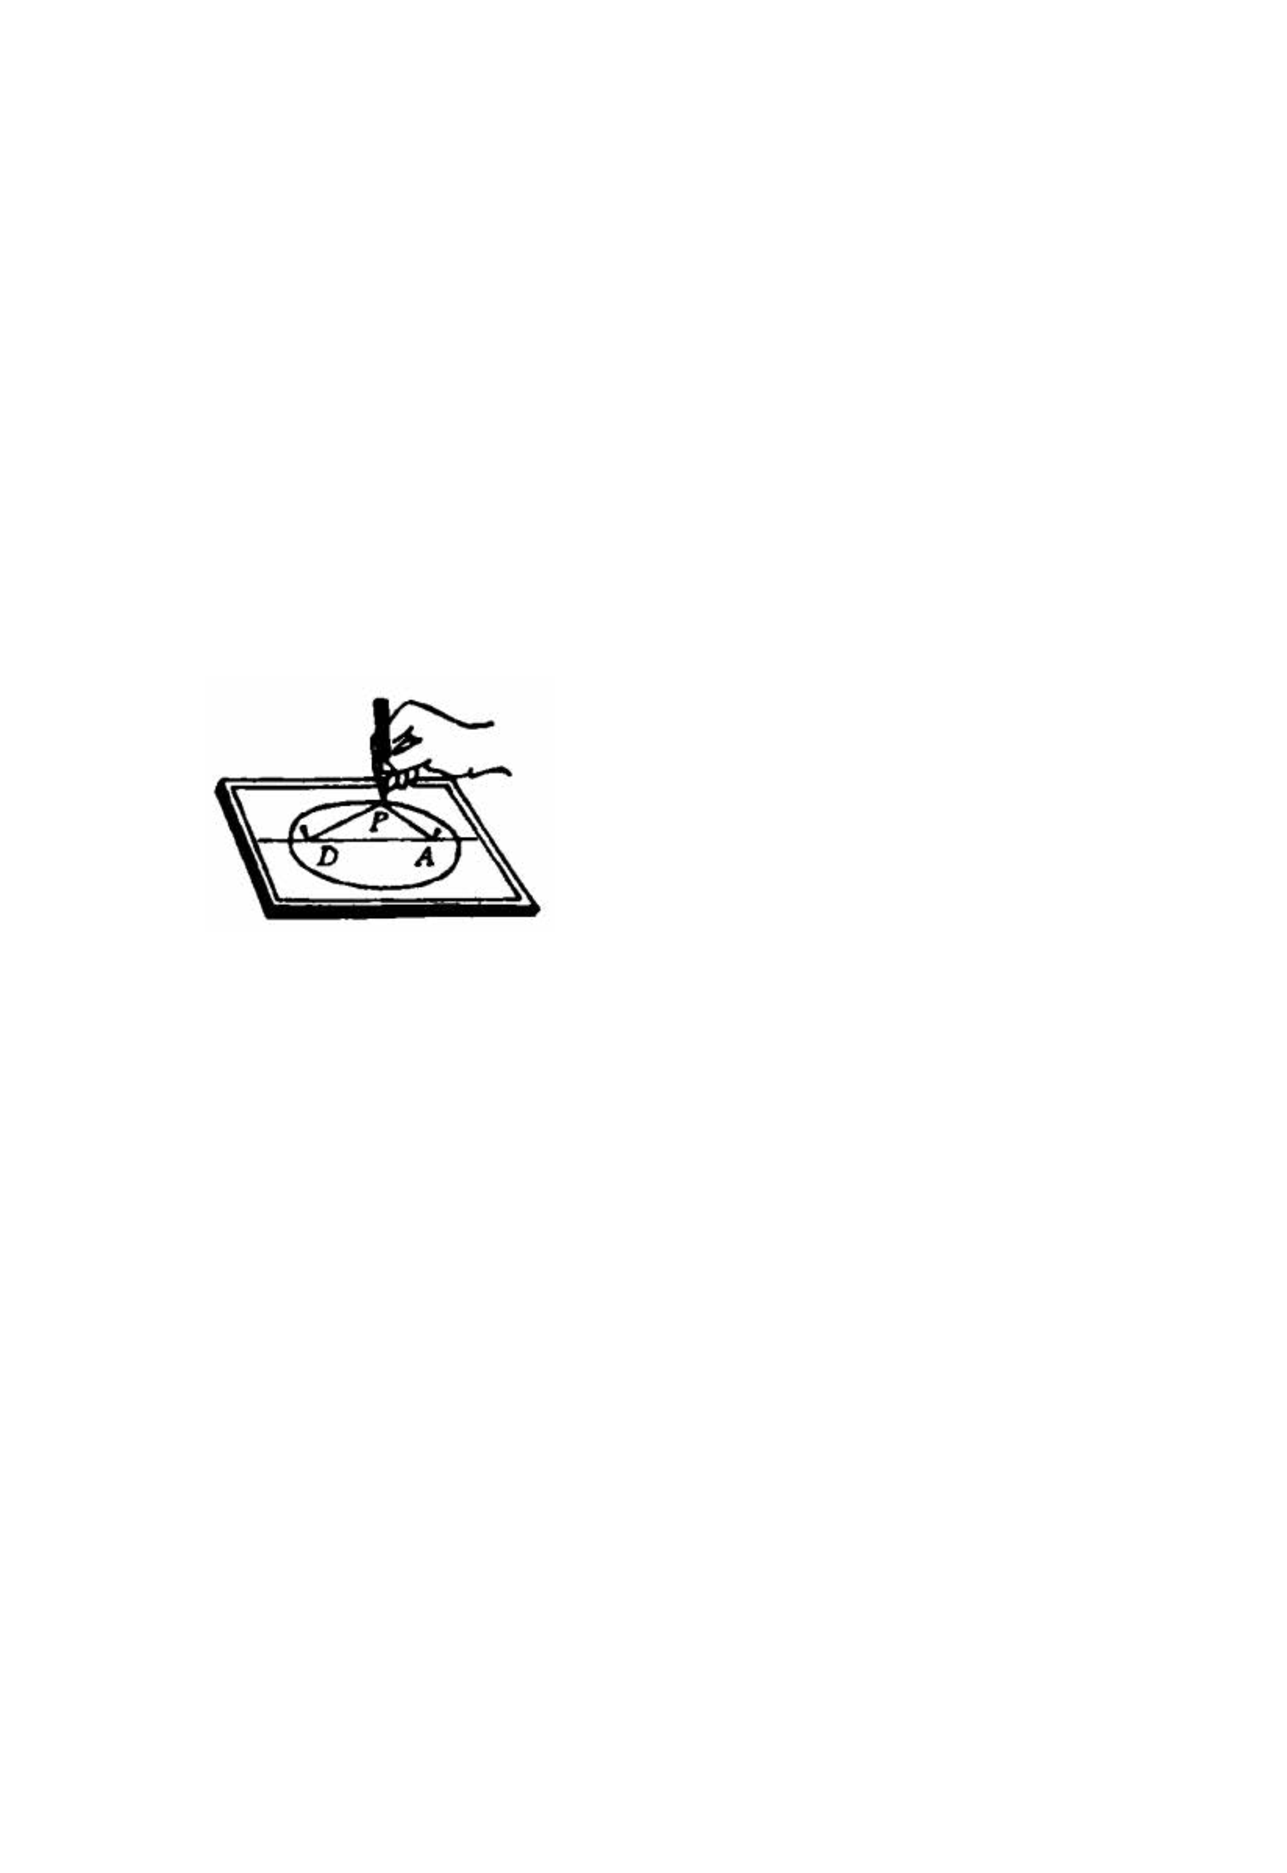
\includegraphics[scale=.8]{fig/3-14.pdf}
    \captionof{figure}{}
\end{minipage}
\hfill
\begin{minipage}{.45\textwidth}
\centering
\begin{tikzpicture}[>=stealth]
\draw[->](-3,0)--(3,0)node[below]{$x$};
\draw[->](0,-1.5)--(0,1.5)node[left]{$y$};
\node[below left]{$O$};
\draw(0,0) ellipse(2 and 1);
\tkzDefPoints{-1.732/0/F_1, 1.732/0/F_2, 1/.866/P}
\tkzLabelPoints[below](F_1,F_2)
\tkzLabelPoints[above](P)
\tkzDrawSegments[dashed](F_1,P P,F_2)

\end{tikzpicture}
\captionof{figure}{}
\end{minipage}

根据椭圆的定义，现在求椭圆的方程.

如图3.15，建立直角坐标系，即以过焦点$F_1$、$F_2$的直线为$x$轴，线段$F_1F_2$的垂直平分线为$y$轴.

设$P(x,y)$是椭圆上任意一点，椭圆的焦距$|F_1F_2|=2c\; (c>0)$，点$P$到$F_1F_2$距离之和为正常数$2a$，则两焦点$F_1,F_2$的坐标分别为$(-c,0)$、$(c,0)$.

$\because\quad |PF1|+|PF2|=2a$

$\therefore\quad \sqrt{(x+c)^2+y^2}+\sqrt{(x-c)^2+y^2}=2a$

将这个方程移项、两边平方，得
\[\begin{split}
    (x+c)^2+y^2&=4a^2-4a\sqrt{(x-c)^2+y^2}+(x-c)^2+y^2\\
    a^2-cx&=a\sqrt{(x-c)^2+y^2}
\end{split} \]
两边再平方，得
\[a^4-2a^2cx+c^2x^2=a^2x^2-2a^2cx+a^2c^2+a^2y^2\]
整理，得
\[(a^2-c^2)x^2+a^2y^2=a^2(a^2-c^2)\]

由椭圆定义可知，$2a>2c$，即$a>c$，所以，$a^2-c^2>0$. 
记$a^2-c^2=b^2\; (b>0)$，得
\[b^2x^2+a^2y^2=a^2b^2\]
两边同除以$a^2b^2$，得
\begin{equation}
    \frac{x^2}{a^2}+\frac{y^2}{b^2}=1\quad (a>b>0) \tag{1}
\end{equation}


\noindent
\begin{minipage}{.63\textwidth}
\CTEXindent
这个方程叫做椭圆的\textbf{标准方程}，它所表示的椭圆的焦点在$x$轴上，两焦点分别是$F_1(-c,0)$、$F_2(c,0)$，这里$c^2=a^2-b^2$.

如果椭圆的焦点在$y$轴上，两焦点分别是$F_1(0,-c)$、$F_2(0,c)$（如图3.16），只要将方程(1)的$x$，$y$互换，就可以得到它的方程，这时方程为
\begin{equation}
    \frac{y^2}{a^2}+\frac{x^2}{b^2}=1\quad (a>b>0) \tag{2}
\end{equation}
这个方程也是椭圆的标准方程.
\end{minipage}
\hfill
\begin{minipage}{.33\textwidth}
\centering
\begin{tikzpicture}[>=stealth]
\draw[->](-2,0)--(2,0)node[below]{$x$};
\draw[->](0,-2.5)--(0,2.5)node[left]{$y$};
\node[below left]{$O$};
\draw[ thick](0,0) ellipse(1 and 2);
\tkzDefPoints{0/-1.732/F_1, 0/1.732/F_2, -.866/-1/P}
\tkzLabelPoints[right](F_1,F_2)
\tkzLabelPoints[left](P)
\tkzDrawSegments[dashed](F_1,P P,F_2)
\end{tikzpicture}
\captionof{figure}{}
\end{minipage}

\begin{example}
    平面内，两个定点的距离是8，试建立适当的坐标系，写出到这两个定点距离之和为10的点的轨迹方程．
\end{example}

\begin{solution}
依椭圆的定义，动点的轨迹是椭圆，两定点是椭圆的焦点，用$F_1$、$F_2$表示. 取过$F_1$、$F_2$的直线为$x$轴，线段$F_1F_2$
的垂直平分线为$y$轴.

由$2a=10,\quad 2c=8\quad \Rightarrow\quad a=5,\quad c=4$
\[b^2=a^2-c^2=5^2-4^2=9 \quad \Rightarrow\quad  b=3\]
$\therefore\quad $椭圆的标准方程是
\[\frac{x^2}{5^2}+\frac{y^2}{3^2}=1\quad \Rightarrow\quad \frac{x^2}{25}+\frac{y^2}{9}=1\]

若取过$F_1F_2$的直线为$y$轴，线段$F_1F_2$的垂直平分线为$x$轴，则这个椭圆的标准方程是
\[\frac{y^2}{25}+\frac{x^2}{9}=1\quad \Rightarrow\quad \frac{x^2}{9}+\frac{y^2}{25}=1\]
\end{solution}

\begin{example}
    求与椭圆$\frac{x^2}{9}+\frac{y^2}{4}=1$共焦点，且过点$M(3,-2)$的椭圆的方程.
\end{example}

\begin{solution}
    \textbf{解法1：} 由已知椭圆的标准方程$\frac{x^2}{9}+\frac{y^2}{4}=1$，得$c^2=9-4=5$, 且焦点在$x$轴上.

设所求椭圆方程为$\frac{x^2}{a^2}+\frac{y^2}{a^2-5}=1$

又$\because\quad $点$M(3,-2)$在椭圆上，
\[\begin{split}
 \therefore\quad \frac{9}{a^2}+\frac{4}{a^2-5}=1\quad \Rightarrow\quad 9(a^2-5)+4a^2&=a^2(a^2-5)\\
a^4-18a^2+45&=0\\
(a^2-15)(a^2-3)&=0.   
\end{split}\]

$\because\quad a^2>c^2=5$

$\therefore\quad $只有$a^2=15$

$\therefore\quad$为所求椭圆的方程.


\textbf{解法2：} 因为所求的椭圆的焦点就是已知椭圆$\frac{x^2}{9}+\frac{y^2}{4}=1$的
两个焦点$F_1(-\sqrt{5},0)$、$F_2(\sqrt{5},0)$. 点$M(3,-2)$到这两个焦点距离之和就是$2a$，即
\[\begin{split}
  2a=|MF_1|+|MF_2|&=\sqrt{\left(3+\sqrt{5}\right)^2+4}+\sqrt{\left(3-\sqrt{5}\right)^2+4}\\
  &=\sqrt{18+6\sqrt{5}}+\sqrt{18-6\sqrt{5}}  \\
  &=\sqrt{\left(\sqrt{15}+\sqrt{3}\right)^2}+\sqrt{\left(\sqrt{15}-\sqrt{3}\right)^2}\\
  &=\left(\sqrt{15}+\sqrt{3}\right)+\left(\sqrt{15}-\sqrt{3}\right)=2\sqrt{15}
\end{split}\]

$\therefore\quad a=\sqrt{15},\quad b^2=a^2-c^2=15-5=10$

$\therefore\quad \frac{x^2}{15}+\frac{y^2}{10}=1$为所求椭圆的方程.
\end{solution}

\subsection*{3.7 练习}
\begin{enumerate}
    \item 写出适合下列条件的椭圆的标准方程：
\begin{enumerate}[(1)]
\item $a=4$、$b=3$，焦点在$x$轴上；
\item $b=1$、$c=\sqrt{15}$，焦点在$y$轴上；
\item 两个焦点分别是$F_1(-2,0)$、$F_2(2,0)$，并且过点$P\left(\frac{5}{2},\; -\frac{3}{2}\right)$.
\end{enumerate}

\item 已知$\triangle ABC$的一边$BC$长为6，周长为16，求顶点$A$的轨迹方程.
\item 设点$P(x_1,y_1)$是椭圆$\frac{x^2}{a^2}+\frac{y^2}{b^2}=1\; (a>b>0)$上的任一点，求
\begin{enumerate}[(1)]
\item 点$P$到椭圆的左焦点$F_1$的距离$|PF_1|$;
\item 点$P$到椭圆的右焦点$F_2$的距离$|PF_2|$;
\item $|PF_1|+|PF_2|$
\end{enumerate}

\item 平面内，到两定点$F_1$、$F_2$距离之和恰为$|F_1F_2|$的动点$P$的轨迹是什么图形？
\end{enumerate}


\section{椭圆的几何性质}
读者可根据椭圆的标准方程
$\frac{x^2}{a^2}+\frac{y^2}{b^2}=1\; (a>b>0)$
来研究椭圆的几何性质. 结论如下：
\begin{enumerate}
    \item 椭圆$\frac{x^2}{a^2}+\frac{y^2}{b^2}=1$有两个焦点$F_1(-C',0)$、$F_2(C',
0)$，（其中$C=\sqrt{a^2-b^2}$）

若点$P$在此椭圆上，则$|PF_1|+|PF_2|=2a$.

\noindent
\begin{minipage}{.45\textwidth}
\item 范围

椭圆$\frac{x^2}{a^2}+\frac{y^2}{b^2}=1$是封闭曲线. 由于$|x|\le a$、$|y|\le b$，因此椭圆位于直线$x=\pm a$, $y=\pm b$所围成的矩形区域内（图3.17）.

\item 对称性

$x$轴、$y$轴是椭圆$\frac{x^2}{a^2}+\frac{y^2}{b^2}=1$的对称轴，原点是此椭圆的对称中心（简称椭圆的\textbf{中心}）.
\end{minipage}
\hfill
\begin{minipage}{.45\textwidth}
\centering
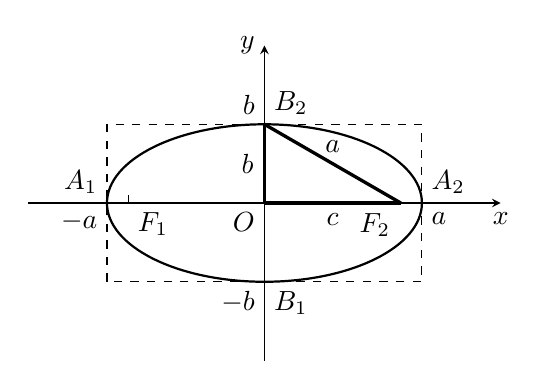
\begin{tikzpicture}[>=stealth]
\draw[->](-3,0)--(3,0)node[below]{$x$};
\draw[->](0,-2)--(0,2)node[left]{$y$};
\node[below left]{$O$};
\draw[thick](0,0)ellipse(2 and 1);
\draw[dashed](-2,-1)rectangle(2,1);
\node at (-2,0)[above left]{$A_1$};
\node at (-2,0)[below left]{$-a$};
\node at (2,0)[above right]{$A_2$};
\node at (2,0)[below right]{$a$};

\draw(-1.732,.1)--(-1.732,0)node[below right]{$F_1$};
\node at (0,1)[above left]{$b$};
\node at (0,1)[above right]{$B_2$};
\node at (0,-1)[below left]{$-b$};
\node at (0,-1)[below right]{$B_1$};

\draw[very thick](0,1)--node[left]{$b$}(0,0);
\draw[very thick](0,1)--node[above]{$a$}(1.732,0)node[below left]{$F_2$};
\draw[very thick](0,0)--node[below]{$c$}(1.732,0);


\end{tikzpicture}
\captionof{figure}{}
\end{minipage}


\item 顶点

令$y=0$，可得椭圆$\frac{x^2}{a^2}+\frac{y^2}{b^2}=1$与其对称轴$x$轴的交点$A_1(-a,0)$、$A_2(a,0)$；令$x=0$，可得此椭圆与它的另一条对称轴$y$轴的交点$B_1(0,-b)$、$B_2(0,b)$. 我们称这四个交点叫做椭圆的\textbf{顶点}.

线段$A_1A_2, B_1B_2$分别叫做椭圆$\frac{x^2}{a^2}+\frac{y^2}{b^2}=1$的\textbf{长轴}和\textbf{短轴}. 并且$|A_1A_2|=2a$, $|B_1B_2|=2a$，正数$a$和$b$分别叫做椭圆$\frac{x^2}{a^2}+\frac{y^2}{b^2}=1$的\textbf{长半轴长}和\textbf{短半轴长}.

\item 离心率

为了刻画椭圆的扁平程度，我们引入一个十分重要的概念.

椭圆的焦距$2c$与长轴长$2a$的比值$\frac{c}{a}$叫做椭圆$\frac{x^2}{a^2}+\frac{y^2}{b^2}=1$的\textbf{离心率}. 记作
$e=\frac{c}{a}$.

$\because\quad 0<c<a,\qquad \therefore\quad 0<e<1$

当$e\to 1$时，$c\to a$，从而$b=\sqrt{a^2-c^2}\to 0$，因此椭圆$\frac{x^2}{a^2}+\frac{y^2}{b^2}=1$越扁；反之，当$e\to 0$时，$c\to 0$，有$b\to a$，这时该椭圆就接近于圆.

不难想象，若$a=b$，则$c=0$，这时原椭圆的两个焦点重合，图形变为圆.
\end{enumerate}

\begin{example}
已知椭圆$\frac{x^2}{a^2}+\frac{y^2}{b^2}=1$（图3.18），填空：
\begin{multicols}{2}
\begin{enumerate}[(1)]
    \item $|F_2A_2|=\blank\blank$;
    \item $|A_1F_2|=\blank\blank$;
    \item $|B_2F_2|=\blank\blank$;
    \item $|A_1F_2|+|A_1F_1|=\blank\blank$;
    \item $|A_1B_2|=\blank\blank$;
    \item 若$|A_1B_2|=|F_1F_2|$，则此椭圆离心率$e=\blank\blank$.
\end{enumerate}    
\end{multicols}

请读者完成.
\end{example}


\noindent
\begin{minipage}{.47\textwidth}
\centering
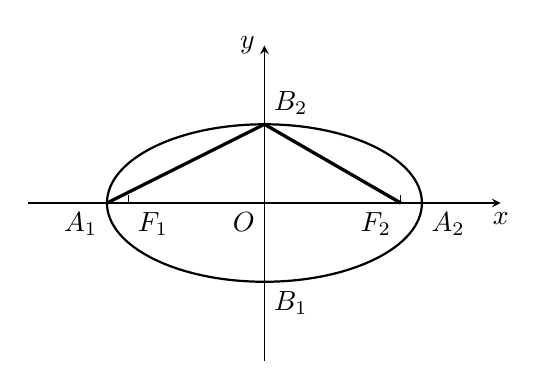
\begin{tikzpicture}[>=stealth]
\draw[->](-3,0)--(3,0)node[below]{$x$};
\draw[->](0,-2)--(0,2)node[left]{$y$};
\node[below left]{$O$};
\draw[thick](0,0)ellipse(2 and 1);
\draw(-1.732,.1)--(-1.732,0)node[below right]{$F_1$};
\draw(1.732,.1)--(1.732,0)node[below left]{$F_2$};
\node at (-2,0)[below left]{$A_1$};
\node at (2,0)[below right]{$A_2$};
\node at (0,1)[above right]{$B_2$};
\node at (0,-1)[below right]{$B_1$};
\draw[very thick](-2,0)--(0,1)--(1.732,0);
\end{tikzpicture}
\captionof{figure}{}
\end{minipage}
\hfill
\begin{minipage}{.47\textwidth}
\centering
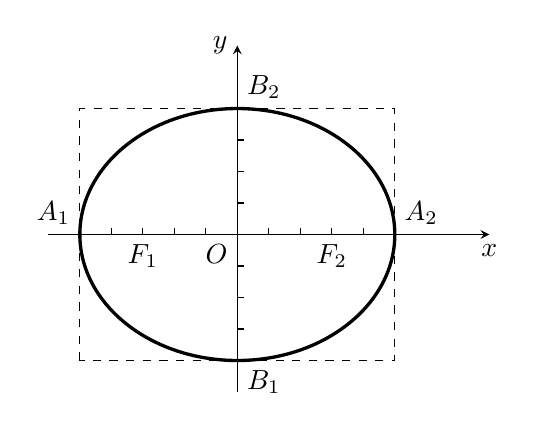
\begin{tikzpicture}[>=stealth, scale=.4]
\draw[->](-6,0)--(8,0)node[below]{$x$};
\draw[->](0,-5)--(0,6)node[left]{$y$};
\node[below left]{$O$};
\draw[very thick](0,0)ellipse(5 and 4);
\draw[dashed](-5,-4) rectangle (5,4);
\node at (-5,0)[above left]{$A_1$};
\node at (5,0)[above right]{$A_2$};
\node at (0,4)[above right]{$B_2$};
\node at (0,-4)[below right]{$B_1$};
\foreach \x in {1,2,3,4}
{
    \draw(\x,0)--(\x,.2);
    \draw(-\x,0)--(-\x,.2);
    \draw(0,\x)--(.2,\x);
    \draw(0,-\x)--(.2,-\x);
}
\node at (3,0)[below]{$F_2$};
\node at (-3,0)[below]{$F_1$};
\tkzDefPoints{0/4/A, 1/3.9/B, 2/3.7/C, 3/3.2/D, 4/2.4/E, 5/0/F}
\tkzDrawPoints(A,B,C,D,E,F)

\end{tikzpicture}
\captionof{figure}{}
\end{minipage}


\begin{example}
求椭圆$16x^2+25y^2=400$
的长轴和短轴的长，离心率，顶点和焦点坐标，并用描点法画出它的图形.
\end{example}

\begin{solution}
    先把已知方程化成标准方程
\[\frac{x^2}{5^2}+\frac{y^2}{4^2}=1\]
这里$a=5$, $b=4$, $c=\sqrt{a^2-b^2}=\sqrt{25-16}=3$

$\therefore\quad$椭圆的长轴长$2a=10$，短轴长$2b=8$，焦距$2c=6$，离心率$e=\frac{c}{a}=\frac{3}{5}$，椭圆的顶点坐标分别是$(\pm 5,0)$和$(0,\pm 4)$，焦点坐标是$(\pm 3,0)$．

将已知方程变形为$y^2=16\left(1-\frac{x^2}{25}\right)$.

当$0\le x\le 5$且$y\ge 0$时，$y=\frac{4}{5}\sqrt{25-x^2}$.
\begin{center}
\begin{tabular}{c|cccccc}
\hline
$x$ & 0  & 1& 2  &3 & 4  &5\\
\hline
$y$ &  4 & 3.9& 3.7  &3.2 & 2.4  &0\\
\hline
\end{tabular}
\end{center}

先用描点法画出椭圆在第一象限内的图形，然后利用椭圆的对称性，画出整个椭圆，如图3.19．
\end{solution}
    
\begin{example}
已知曲线$c$的方程为$\frac{x^2}{9-k}+\frac{y^2}{k-1}=1\; (1<k<9)$，试根据$k$的不同取值，确定曲线$C$是什么曲线？
\end{example}

\begin{solution}
    $\frac{x^2}{9-k}+\frac{y^2}{k-1}=1\quad (1<k<9)$
\begin{enumerate}[(1)]
    \item  当$9-k=k-1$即$k=5$时，曲线$C$是圆$x^2+y2=4$（其中圆心为原点$O$，半径$r=2$）
    \item  当$9-k>k-1>0$即$1<k<5$时，
\[\begin{cases}
    a^2=9-k\\ b^2=k-1
\end{cases}\Rightarrow c^2=a^2-b^2=10-2k\]
    曲线$C$是以$F_1\left(-\sqrt{10-2k},0\right)$、$F_2\left(\sqrt{10-2k},0\right)$为焦点，$a=\sqrt{9-k}$的椭圆.
    \item  当$0<9-k<k-1$即$5<k<9$时，
    \[\begin{cases}
        a^2=k-1\\ b^2=9-k
    \end{cases}\Rightarrow c^2=a^2-b^2=2k-10\]
    曲线$C$是以$F_1\left(0,-\sqrt{2k-10}\right)$、$F_2\left(0,\sqrt{2k-10}\right)$为焦点，$a=\sqrt{k-1}$的椭圆.
 \end{enumerate}
\end{solution}

椭圆除有上述几何性质外，还有一个很重要的性质. 我们先看一个具体的例子.   

\begin{example}
    点$M(x,y)$与定点$F(c,0)$的距离和它到定直线$\ell:\; x=\frac{a^2}{c}$的距离的比是常数$\frac{c}{a}\; (a>c>0)$. 求点$M$的轨迹.
\end{example}

\begin{solution}
设$d$是点$M$到直线$\ell$的距离. 根据题意，所求轨迹就是集合
\[P=\left\{\text{点}M\Big|\frac{|MF|}{d_{M-\ell}}=\frac{c}{a}\right\}\]
由此得

\noindent
\begin{minipage}{.45\textwidth}
\[\frac{\sqrt{(x-c)^2+y^2}}{\left|\frac{a^2}{c}-x\right|}=\frac{c}{a}\]
将上式化简，得
\[(a^2-c^2)x^2+a^2y^2=a^2(a^2-c^2)\]

设$a^2-c^2=b^2$，就可化成
\[\frac{x^2}{a^2}+\frac{y^2}{b^2}=1\]
\end{minipage}
\hfill
\begin{minipage}{.52\textwidth}
\centering
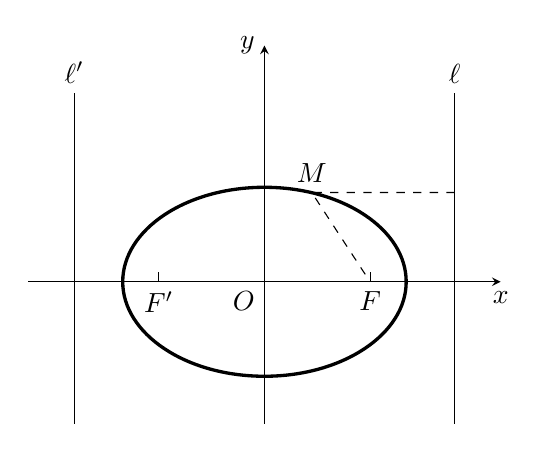
\begin{tikzpicture}[>=stealth, scale=.6]
\draw[->](-5,0)--(5,0)node[below]{$x$};
\draw[->](0,-3)--(0,5)node[left]{$y$};
\node[below left]{$O$};
\draw[very thick](0,0) ellipse (3 and 2);
\draw(-2.236,0)node[below]{$F'$}--(-2.236,.2);
\draw(2.236,0)node[below]{$F$}--(2.236,.2);
\foreach \x/\y in {4.025/\ell,-4.025/\ell'}
{
    \draw(\x, -3)--(\x, 4)node[above]{$\y$};
}
\draw[dashed](4.025,1.89)--(1,1.89)node[above]{$M$}--(2.236,0);

\end{tikzpicture}
\captionof{figure}{}
\end{minipage}

这是椭圆的标准方程，所以点$M$的轨迹是椭圆（图3.20）．
\end{solution}


由上面的例子可知，点$M$与一个定点的距离和它到一条定直线的距离的比是常数$e=\frac{c}{a}\; (e<1)$时，这个点的轨迹是椭圆. 由此，我们也可这样定义椭圆：
\begin{thm}
    {定义} 平面内，到一定点$F$和一条定直线$\ell$的距离之比是一个常数$e\; (0<e<1)$的动点$P$的轨迹叫做\textbf{椭圆}. 这个定点叫做椭圆的一个焦点，定直线叫做相应于这个焦点的椭圆的准线，$e$叫做椭圆的离心率. 线段$FP$叫做椭圆的\textbf{焦半径}.
\end{thm}




\noindent
\begin{minipage}{.45\textwidth}\CTEXindent
    对于椭圆$\frac{x^2}{a^2}+\frac{y^2}{b^2}=1$来说，相应于右焦点$F(c,0)$的准线方程为$x=\frac{a^2}{c}$，根据椭圆的对称性，相应于左焦点$F'(-c,0)$的准线方程是$x=-\frac{a^2}{c}$，所以椭圆
    有两条准线（图3.21）．
\end{minipage}
\hfill
\begin{minipage}{.5\textwidth}
\centering
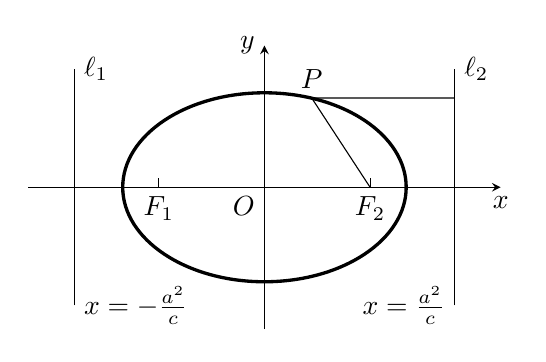
\begin{tikzpicture}[>=stealth, scale=.6]
\draw[->](-5,0)--(5,0)node[below]{$x$};
\draw[->](0,-3)--(0,3)node[left]{$y$};
\node[below left]{$O$};
\draw[very thick](0,0) ellipse (3 and 2);
\draw(-2.236,0)node[below]{$F_1$}--(-2.236,.2);
\draw(2.236,0)node[below]{$F_2$}--(2.236,.2);
\draw(4.025, -2.5)node[left]{$x=\frac{a^2}{c}$}--(4.025, 2.5)node[right]{$\ell_2$};
\draw(-4.025, -2.5)node[right]{$x=-\frac{a^2}{c}$}--(-4.025, 2.5)node[right]{$\ell_1$};
\draw[](4.025,1.89)--(1,1.89)node[above]{$P$}--(2.236,0);
\tkzDefPoints{1/1.89/A, 4.025/1.89/B, 4.025/2/C}
\tkzMarkRightAngles[size=.2](A,B,C)
\end{tikzpicture}
\captionof{figure}{}
\end{minipage}

设椭圆$\frac{x^2}{a^2}+\frac{y^2}{b^2}=1$上
的任意一点$P$到右准线$\ell:\; x=\frac{a^2}{c}$的距离为$d_{P-\ell}$, 
根据椭圆的第二定义，得
\[\frac{|PF_2|}{d_{P-\ell}}=e\]

$\therefore\quad |PF_2|=ed_{P-\ell}=e\left(\frac{a^2}{c}-x\right)=a-ex$

同理可求，$|PF_1|=a+ex$.





\begin{example}
    设$P$是椭圆$\frac{x^2}{25}+\frac{y^2}{16}=1$一点，若它到椭圆的右焦点$F_2$的距离为4，求它到椭圆的左准线的距离$d_1$的值.
\end{example}

\begin{solution}
\textbf{解法1：}由$\frac{x^2}{25}+\frac{y^2}{16}=1$得$a=5,\; b=4,\; c=3$.

\noindent
\begin{minipage}{.53\textwidth}\CTEXindent
连结$PF_1$，作$PE_1\bot $左准线于$E_1$，则$d_1=|PE_1|$.

$\because\quad |PF_1|+|PF_2|=2a $

$\therefore\quad |PF|=2a-|PF_1|=10-4=6$.

又$\because\quad \frac{|PF_1|}{d_1}=e$
\end{minipage}
\hfill
\begin{minipage}{.45\textwidth}
\centering
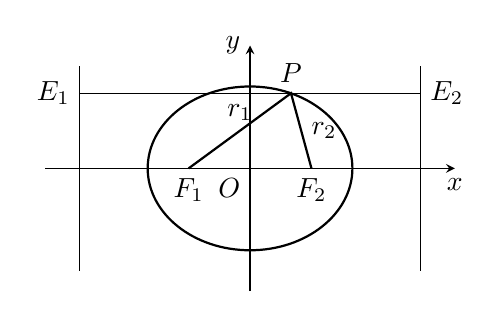
\begin{tikzpicture}[>=stealth, scale=.26]
\draw[->](-10,0)--(10,0)node[below]{$x$};
\draw[->](0,-6)--(0,6)node[left]{$y$};
\node[below left]{$O$};
\draw[thick](0,0) ellipse (5 and 4);
\draw(8.33,-5)--(8.33,5);
\draw(-8.33,-5)--(-8.33,5);
\draw[thick](-3,0)node[below]{$F_1$}--node[above]{$r_1$}(2,3.67)node[above]{$P$}--node[right]{$r_2$}(3,0)node[below]{$F_2$};
\draw(-8.33,3.67)node[left]{$E_1$}--(8.33,3.67)node[right]{$E_2$};

\end{tikzpicture}
\captionof{figure}{}
\end{minipage}

$\therefore\quad d_1=\frac{|PF_1|}{e}=\frac{|PF_1|}{\frac{c}{a}}=6\x \frac{5}{3}=10$


\textbf{解法2：}过$P$点作椭圆$\frac{x^2}{25}+\frac{y^2}{16}=1$的两准线的垂直线段$E_1E_2$（图3.22），则$d_1=|PE_1|$, $d_2=|PE_2|$.

$\because\quad \frac{|PF_2|}{|PE_2|}=e$

$\therefore\quad d_2=|PE_2|=\frac{|PF_2|}{e}=\frac{4}{e}=4\x \frac{5}{3}$

又$\because\quad d_1+d_2=2\cdot  \frac{a^2}{c}$

$\therefore\quad d_1=2\cdot \frac{a^2}{c}-d_2=2\x \frac{25}{3}-4\x\frac{5}{3}=\frac{10}{3}\cdot (5-2)=10$
\end{solution}

\begin{example}
    已知$F_1$、$F_2$是椭圆$\frac{x^2}{100}+\frac{y^2}{64}=1$的两个焦点，$P$是椭圆上一点，且$\angle F_1PF_2=\frac{2\pi}{3}$，求三角形$F_1PF_2$的面积（图3.23）．
\end{example}

\begin{solution}
设$|PF_1|=m$, $|PF_2|=n$.

$\because \quad S_{\triangle F_1PF_2}=\frac{1}{2}mn\sin\frac{2\pi}{3}=\frac{\sqrt{3}}{4}mn$

$\therefore\quad $欲求$S_{\triangle F_1PF_2}$，只需求$mn$的积.

由已知椭圆方程$\frac{x^2}{100}+\frac{y^2}{64}=1$，知$a=10,\; b=8,\; c=6$

\noindent
\begin{minipage}{.57\textwidth}
\[\begin{split}
\because\quad &\begin{cases}
    m+n=2a=20\\
    m^2+n^2-2mn\cos\frac{2\pi}{3}=|F_1F_2|^2=4c^2=144
\end{cases}\\
& \Rightarrow \begin{cases}
    (m+n)^2=400\\
    m^2+n^2+mn=144
\end{cases}    
\end{split} \]

$\therefore\quad mn=256$

$S_{\triangle F_1PF_2}=\frac{\sqrt{3}}{4}\x 256=64\sqrt{3}$
\end{minipage}
\hfill
\begin{minipage}{.4\textwidth}
\centering
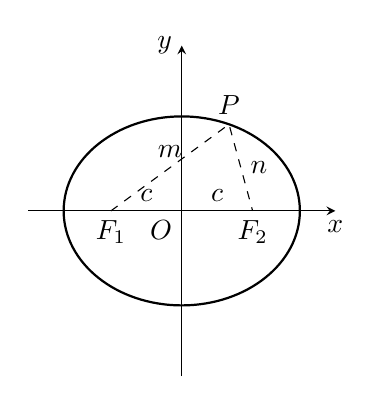
\begin{tikzpicture}[>=stealth, scale=.15]
\draw[->](-13,0)--(13,0)node[below]{$x$};
\draw[->](0,-14)--(0,14)node[left]{$y$};
\node[below left]{$O$};
\draw[thick](0,0) ellipse (10 and 8);
\node at (3,0)[above]{$c$};
\node at (-3,0)[above]{$c$};
\draw[dashed](-6,0)node[below]{$F_1$}--node[above]{$m$}(4,7.33)node[above]{$P$}--node[right]{$n$}(6,0)node[below]{$F_2$};

\end{tikzpicture}
\captionof{figure}{}
\end{minipage}


\end{solution}

\subsection*{3.8 练习}
\begin{enumerate}
    \item 根据下列条件，求椭圆的标准方程：
\begin{enumerate}[(1)]
\item 中心在原点，焦点在$x$轴上，长短轴分别是8和6；
\item 中心在原点，一个焦点坐标为$(0,5)$，短轴长是4；
\item 长短轴都在坐标轴上，且经过点$P(-2,0)$和$Q(0,-3)$;
\item 长短轴都在坐标轴上，半长轴等于10，离心率等于0.6；
\item 长短轴都在坐标轴上，且长轴是短轴的3倍且过点$P(3,0)$;
\item 椭圆关于两个坐标轴对称，长短轴的长之和是20，焦距是$4\sqrt{5}$.
\end{enumerate}

\item 我国发射的科学试验人造地球卫星运行的轨道是以地球的
    中心为一个焦点的椭圆，近地点距地面266千米，远地点距地面1826千米，求卫星的轨道方程（地球半径为6370公里）.
    \item 填空：
\begin{center}
\begin{tabular}{c|cc}
    \hline
椭圆方程&$9x^2+y^2=81$&$x^2+4y^2=16$\\
\hline
标准方程\\
长轴的长\\
短轴的长\\
离心率$e$\\
焦点坐标\\
顶点坐标\\
准线方程\\
\hline
\end{tabular}
\end{center}

\item 若椭圆$\frac{x^2}{a^2}+\frac{y^2}{b^2}=1\; (a>b>0)$的两个焦点将其两准线间的
且与准线垂直的线段三等分，
\begin{enumerate}[(1)]
\item 求离心率$e$；
\item 若点$(3,-2)$在此椭圆上，求椭圆的标准方程．
\end{enumerate}

\item 求中心在原点，长轴在$y$轴，离心率$e=\frac{\sqrt{5}}{3}$，一条准线的方程是$y=-3$的椭圆方程.
\end{enumerate}

\section{椭圆的参数方程}
大家知道，引入曲线的参数方程的价值在于，借助参数可较简单地表示曲线上任意一点的坐标.学习了椭圆的标准方程后自然会想到，椭圆的参数方程如何构造？参数选什么量合适？由于$\frac{x^2}{a^2}+\frac{y^2}{b^2}=1$可以写成$\left(\frac{x}{a}\right)^2+\left(\frac{y}{b}\right)^2=1$，这后一方程的结构特征与我们十分熟悉的三角公式$\cos^2\alpha+\sin^2\alpha=1$的结构相同，这就“启示”我们不妨令
\[\begin{cases}
    \frac{x}{a}=\cos\varphi \\[1.5ex]
    \frac{y}{b}=\sin\varphi 
\end{cases}(\varphi\in\R)\quad \text{即}\quad \begin{cases}
    x=a\cos\varphi\\
    y=b\sin\varphi\\
\end{cases}(\varphi\in\R)\]

求证：方程$\begin{cases}
    x=a\cos\varphi\\
    y=b\sin\varphi\\
\end{cases}(\varphi\in\R)$是椭圆$\frac{x^2}{a^2}+\frac{y^2}{b^2}=1$的参数方程.

\begin{proof}
在椭圆上任取一点$P(x_1,y_1)$，则
\[\frac{x_1^2}{a^2}+\frac{y_1^2}{b^2}=1 \quad \text{即} \left(\frac{x_1}{a}\right)^2+\left(\frac{y_1}{b}\right)^2=1\]
这就是说点$\left(\frac{x_1}{a},\; \frac{y_1}{b}\right)$是单位圆上的一点，从而总存在一个角$\varphi_1$，使得
\[\begin{cases}
    \frac{x_1}{a}=\cos\varphi_1 \\[1.5ex]
    \frac{y_1}{b}=\sin\varphi_1 
\end{cases}\Rightarrow \quad \begin{cases}
    x_1=a\cos\varphi_1\\
    y_1=b\sin\varphi_1\\
\end{cases}\]

$\therefore\quad $点$P(x_1,y_1)$在方程$\begin{cases}
    x=a\cos\varphi\\
    y=b\sin\varphi\\
\end{cases}(\varphi\in\R)$的曲线上.

另一方面，由于上述每步都可逆，即任取$\theta'\in\R$，由关系式$\begin{cases}
    x'=a\cos\theta'\\
    y'=b\sin\theta'\\
\end{cases}$，所确定的点$P(x',y')$都必在椭圆$\frac{x^2}{a^2}+\frac{y^2}{b^2}=1$上.

$\therefore\quad $方程$\begin{cases}
    x=a\cos\varphi\\
    y=b\sin\varphi\\
\end{cases}(\varphi\in\R)$是椭圆$\frac{x^2}{a^2}+\frac{y^2}{b^2}=1$的参数方程.

有了椭圆的参数方程，今后再画椭圆$\frac{x^2}{a^2}+\frac{y^2}{b^2}=1$上的点就十分简便了．如图3.24：

\noindent
\begin{minipage}{.48\textwidth}\CTEXindent
以原点为圆心，分别以$a, b\; (a>b)$为半径作两个圆. 点$B$是大圆半径与小圆的交点，过点$A$作$AN\bot Ox$，垂足为$N$，过点$B$作$BM\bot AN$，垂足为$M$. 则$M$就是椭圆$\frac{x^2}{a^2}+\frac{y^2}{b^2}=1$上的一点（其中$\angle AOX=\varphi$叫做\textbf{离心角}），如图3.24. 有了椭圆的参数方程，还为解决有关椭圆的问题带来不少方便.
\end{minipage}
\hfill
\begin{minipage}{.5\textwidth}
\centering
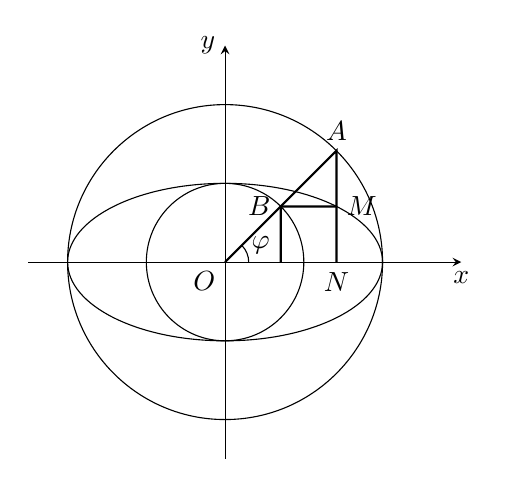
\begin{tikzpicture}[>=stealth]
\draw[->](-2.5,0)--(3,0)node[below]{$x$};
\draw[->](0,-2.5)--(0,2.75)node[left]{$y$};
\node[below left]{$O$};
\draw(0,0)ellipse(2 and 1);
\draw(0,0)circle(2);
\draw(0,0)circle(1);
\draw[thick](0,0)--(45:1)node[left]{$B$}--(45:2)node[above]{$A$}--(1.414,0)node[below]{$N$};
\draw[thick](0.707,0)--(45:1)--+(0.707,0)node[right]{$M$};
\draw(.3,0) arc (0:45:.3)node[right]{$\varphi$};
\end{tikzpicture}
\captionof{figure}{}
\end{minipage}
\end{proof}

\begin{example}
    设$O$是坐标系原点，$P$是椭圆$\begin{cases}
        x=3\cos\varphi\\
        y=2\sin\varphi\\
    \end{cases}$上$\varphi=\frac{\pi}{6}$的一点，求直线$OP$的倾角$\alpha$.
\end{example}

\begin{solution}
当$\varphi=\frac{\pi}{6}$时，

$\because\quad \begin{cases}
    x_p=3\cos\frac{\pi}{6}=\frac{3\sqrt{3}}{2}\\[1.5ex]
    y_p=2\sin\frac{\pi}{6}=1
\end{cases}$

$\therefore\quad k_{op}=\frac{y_p}{x_p}=\frac{2}{3\sqrt{3}}=\frac{2\sqrt{3}}{9},\quad \alpha=\arctan \frac{2\sqrt{3}}{9}$

 特别注意的是，直线$OP$的倾角$\alpha$与椭圆参数方程
$\begin{cases}
    x=3\cos\varphi\\ y=2\sin\varphi
\end{cases}$    中的离心角$\varphi$不等.
\end{solution}



\begin{example}
    求椭圆$\frac{x^2}{a^2}+\frac{y^2}{b^2}=1$中内接矩形的面积$S$的最大值（图3.25）．
\end{example}

\begin{solution}
设$P(x,y)$是椭圆$\frac{x^2}{a^2}+\frac{y^2}{b^2}=1$上位于第一象限内的任一点，则

\noindent
\begin{minipage}{.52\textwidth}
\[\begin{cases}
    x=a\cos\varphi\\ y=b\sin\varphi
\end{cases}\left(0<\varphi<\frac{\pi}{2}\right)\]

由椭圆的对称性，不难得出
\[\begin{split}
    S=4xy&=4ab\cos\varphi \sin\varphi\\
    &=2ab\sin2\varphi\\
    &\le 2ab
\end{split} \]
\end{minipage}
\hfill
\begin{minipage}{.45\textwidth}
\centering
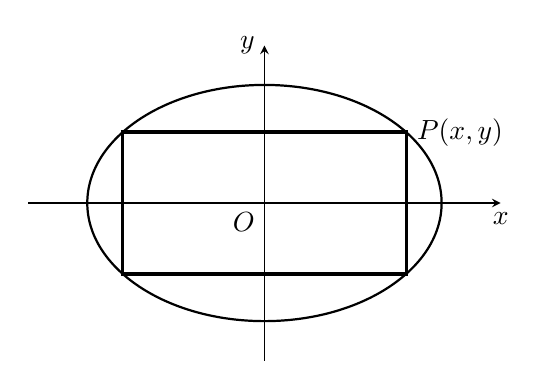
\begin{tikzpicture}[>=stealth]
\draw[->](-3,0)--(3,0)node[below]{$x$};
\draw[->](0,-2)--(0,2)node[left]{$y$};
\node[below left]{$O$};
\draw[thick](0,0)ellipse(2.25 and 1.5);
\draw[very thick](-1.8,-.9)rectangle(1.8,.9)node[right]{$P(x,y)$};

\end{tikzpicture}
\captionof{figure}{}
\end{minipage}

（当且仅当$\sin2\varphi=1$，即$\varphi=\frac{\pi}{4}$时，取等号）

$\therefore\quad S$的最大值为$2ab$．
\end{solution}

\begin{example}
    若圆$(x-1)^2+y^2=r^2$与椭圆$\frac{x^2}{4}+y^2=1$有公共点，求$r^2$的取值范围.
\end{example}

\begin{solution}
椭圆$\frac{x^2}{4}+y^2=1$的参数方程为
\[\begin{cases}
    x=2\cos\varphi\\
    y=\sin\varphi
\end{cases}(\varphi\in\R)\]

$\because\quad $此椭圆与圆$(x-1)^2+y^2=r^2$有公共点，
\[\begin{split}
    \therefore\quad r^2=(2\cos\varphi -1)^2+(\sin\varphi)^2&=3\cos^2\varphi-4\cos\varphi+2\\
&=3\left(\cos\varphi-\frac{2}{3}\right)^2+\frac{2}{3}
\end{split}\]
\begin{itemize}
    \item 当$\cos\varphi=-1$时，$r^2$有最大值9；
    \item 当$\cos\varphi=\frac{2}{3}$时，$r^2$有最小值$\frac{2}{3}$.
\end{itemize}

$\therefore\quad \frac{2}{3}\le r^2\le 9$.
\end{solution}

\subsection*{3.9 练习}
\begin{enumerate}
\item 设$x=b\cos\theta$（$\theta$是参数），求椭圆$\frac{x^2}{b^2}+\frac{y^2}{a^2}=1$的参数方程.
\item 已知点$P(x,y)$是椭圆$\frac{x^2}{4}+y^2=1$上的动点，求$2x+y$的最大值和最小值.
\item 设$y=tx+4$（$t$为参数），求椭圆$4x^2+y^2=16$的参数方程.
\end{enumerate}

\section{椭圆与直线的位置关系}
像直线与圆的位置关系一样，一条直线与已知椭圆的位置关系也有三种，它们之间无公共点、有一个公共点、有两个公共点.

当直线与椭圆有两个公共点时，称直线与椭圆相交. 直线被椭圆所截得的线段又称为椭圆的弦.

本节主要研究直线与椭圆相交时的有关问题.



\begin{example}
    当$m$为何值时，直线$y=x+m$与椭圆$\frac{x^2}{16}+\frac{y^2}{9}=1$相交？
\end{example}

\begin{solution}
\[\begin{cases}
    y=x+m &(1)\\
    9x^2+16y^2=16\x 9&(2)
\end{cases}\]
(1)代入(2)
\[9 x^2+16(x+m)^2-16\x9=0\]
整理得
\begin{equation}
    25x^2+32mx+16(m^2-9)=0 \tag{3}
\end{equation}

$\therefore\quad \Delta =64[16m^2-25(m^2-9)]=576(25-m^2)$

$\therefore\quad $当$25-m^2>0$即$|m|<5$时，$\Delta>0$；方程(3)有两个不等实根，使原方程组有两组不同的实数解.

$\therefore\quad $当$-5<m<5$时，直线$y=x+m$与椭圆$\frac{x^2}{16}+\frac{y^2}{9}=1$相交.
\end{solution}

\begin{remark}
    本题是利用一元二次方程的判别式值的正负，确定直线与椭圆的位置关系. 不难概括出：
\begin{itemize}
    \item $\Delta >0 \Longleftrightarrow$直线与椭圆有两个交点（相交）；
    \item $\Delta =0 \Longleftrightarrow$直线与椭圆只有一个公共点（相切）；
    \item $\Delta <0 \Longleftrightarrow$直线与椭圆无公共点（相离）.
\end{itemize}
\end{remark}

\begin{example}
求直线$y=2x-4$被椭圆$\frac{4x^2}{9}+\frac{y^2}{9}=1$所截的弦$AB$的长.
\end{example}

\begin{solution}
\textbf{解法1：}
\[\begin{cases}
    y=2x-4&(1)\\
    4x^2+y^2=9&(2)
\end{cases}\]
(1)代入(2)
\[\begin{split}
    4x^2+(2x-4)^2&=9\\
8x^2-16x+7&=0\\
x=\frac{16\pm\sqrt{32}}{16}&=1\pm\frac{1}{4}\sqrt{2}
\end{split}\]

$\therefore\quad \begin{cases}
    x_1=1+\frac{1}{4}\sqrt{2}\\[1.5ex]
    y_1=-2+\frac{1}{2}\sqrt{2}
\end{cases} \qquad \begin{cases}
    x_2=1-\frac{1}{4}\sqrt{2}\\[1.5ex]
    y_2=-2-\frac{1}{2}\sqrt{2}
\end{cases}$

\[|AB|=\sqrt{(x_2-x_1)^2+(y_2-y_1)^2}=\sqrt{\left(\frac{1}{2}\sqrt{2}\right)^2+\left(\sqrt{2}\right)^2}=\frac{\sqrt{10}}{2}\]

$\therefore\quad $直线$y=2x-4$被椭圆$\frac{4x^2}{9}+\frac{y^2}{9}=1$所截的弦$AB$的长为$\frac{\sqrt{10}}{2}$.


\begin{analyze}
    对于这类求弦长的问题能否不求直线与椭圆交点的坐标，而找到一个求弦长的计算关系式？

$\because\quad y=kx+b$.

$\therefore\quad y_2-y_1=k(x_2-x_1)$
\[\begin{split}
    \therefore\quad |AB|=\sqrt{(x_2-x_1)^2+(y_2-y_1)^2}&=\sqrt{(x_2-x_1)^2+k^2(x_2-x_1)^2}\\
    &=\sqrt{1+k^2}\sqrt{(x_2-x_1)^2}\\
    &=\sqrt{1+k^2}|x_2-x_1|
\end{split}\]

若$x_1$、$x_2$是二次方程$Ax^2+Bx+C=0$的两个根，则由求根公式不难得出
\[|x_2-x_1|=\frac{\sqrt{B^2-4AC}}{|A|}\]
\end{analyze}


\textbf{解法2：}
\[\begin{cases}
    y=2x-4&(1)\\
    4x^2+y^2=9&(2)
\end{cases}\]
(1)代入(2)化简得：$8x^2-16x+7=0$

$\therefore\quad |AB|=\sqrt{1+k^2}\cdot |x_2-x_1|=\sqrt{1+2^2}\x \frac{\sqrt{\Delta}}{8}=\sqrt{5}\x \frac{\sqrt{32}}{8}=\frac{\sqrt{10}}{2}$
\end{solution}


\begin{example}
    求椭圆$\frac{x^2}{8}+\frac{y^2}{5}=1$内以$A(2,-1)$点为中点的弦所在的直线方程.
\end{example}

\begin{solution}
\textbf{解法1：}
设直线$y+1=k(x-2)$为所求，则
\[\begin{cases}
    y=kx-(2k+1)&(1)\\
    5x^2+8y^2=40&(2)
\end{cases}\]
(1)代入(2)，得
\[5x^2+8[kx-(2k+1)]^2=40\]
整理得
\[(8k^2+5)x^2-16k(2k+1)x+8[(2k+1)^2-5]=0\]

$\because\quad A$点在已知椭圆内，

$\therefore\quad \Delta>0$.

设弦的两端点的横坐标为$x_1,x_2$，
则
\[ \begin{split}
    4=x_1+x_2&=\frac{16k(2k+1)}{8k^2+5}\\
8k^2+5&=4k(2k+1)\\
4k&=5 \quad\Rightarrow \quad k=\frac{5}{4}
\end{split} \]

$\therefore\quad y=\frac{5}{4}x-\frac{7}{2}$即$5x-4y-14=0$为所求.

\textbf{解法2：}
设所求直线的参数方程为$\begin{cases}
    x=2+t\cos\alpha\\ y=-1+t\sin\alpha
\end{cases}$将它代入已
知椭圆方程$5x^2+8y^2=40$，得
\[5(2+t\cos\alpha)^2+8(-1+t\sin\alpha)^2-40=0\]
整理得
\[(5+3\sin^2\alpha)t^2+4(5\cos\alpha-4\sin\alpha)t-12=0\]

$\because\quad $点$A(2,-1)$是弦的中点，

$\therefore\quad \frac{-4(5\cos\alpha-4\sin\alpha)}{5+3\sin^2\alpha}=0$，即$5\cos\alpha-4\sin\alpha=0$

$\therefore\quad k=\tan\alpha=\frac{5}{4}$

$\therefore\quad $所求的直线方程为$y+1=\frac{5}{4}(x-2)$，即$5x-4y-14=0$.

\textbf{解法3：}
设点$P(x,y)$是椭圆$5x^2+8y^2=40$上一点，它关于点$A(2,-1)$的对称点$P'(4-x,-2-y)$恰好在此椭圆上，
则
\[\begin{cases}
    5(4-x)^2+8(-2-y)^2=40 & (1)\\
    5x^2+8y^2=40&(2)
\end{cases}\]
$(1)-(2)$得
\[5(16-8x)+8(4+4y)=0\]
整理得
\[5x-4y-14=0\]

\textbf{解法4：}
设直线$y+1=k(x-2)$与椭圆$5x^2+8y^2=40$的交点为$M(x_1,y_1)$、$N(x_2,y_2)$，且$|MA|=|NA|$. 则
\[\begin{cases}
    5x_1^2+8y^2_1=40&(1)\\
    5x^2_2+8y^2_2=40&(1)\\
    x_1+x_2=4&(3)\\
    y_1+y_2=-2&(4)
\end{cases}\]
$(2)-(1)$得
\[\begin{split}
   5(x_2^2-x_1^2)+8(y_2^2-y_1^2)&=0\\
5(x_2-x_1)(x_2+x_1)+8(y_2-y_1)(y_2+y_1)&=0\\
20(x_2-x_1)-16(y_2-y_1)&=0 
\end{split}\]

$\because\quad k=\frac{y_2-y_1}{x_2-x_1}=\frac{5}{4}$,

$\therefore\quad$所求直线为$y+1=\frac{5}{4}(x-2)$，即$5x-4y-14=0$.
\end{solution}

\begin{remark}
本题给出了四种解法. 请读者自己总结一下各个解法的基本思路及方法，并能运用这些方法解决今后遇到的问题.
\end{remark}

\begin{example}
    求椭圆$\frac{x^2}{100}+\frac{y^2}{25}=1$上一动点$P$到直线$3x+8y+72=0$
距离的最大值及最小值.
\end{example}

\begin{solution}
\textbf{解法1：}因为点$P(x,y)$在椭圆$\frac{x^2}{100}+\frac{y^2}{25}=1$上，所以
\[\begin{cases}
    x_p=10\cos\varphi\\
    y_p=5\sin\varphi\\
\end{cases}(\varphi\in\R)\]
则点$P$到直线$3x+8y+72=0$的距离为
\[\begin{split}
    d&=\frac{|30\cos\varphi+40\sin\varphi+72|}{\sqrt{9+64}}\\
    \theta=\arctan\frac{3}{4}\to &=\frac{|50\sin(\varphi+\theta)+72|}{\sqrt{73}}
\end{split}\]
\begin{itemize}
    \item 当$\sin(\varphi+\theta)=1$时，$d_{\max}=\frac{122}{\sqrt{73}}=\frac{122\sqrt{73}}{73}$
\item 当$\sin(\varphi+\theta)=-1$时，$d_{\min}=\frac{22}{\sqrt{73}}=\frac{22\sqrt{73}}{73}$
\end{itemize}

\textbf{解法2：}分析如果我们把直线$3x+8y+72=0$平行移动，使其与椭圆有公共点$P$，则二平行线间的距离即是椭圆上动点$P$到直线$3x+8y+72=0$的距离. 因而可得下面解法：

设与直线$3x+8y+72=0$平行的直线为$3x+8y+t=0$.
\[\begin{cases}
    8y=-3x-t\\
    16x^2+64y^2=1600
\end{cases}\Rightarrow 16x^2+(3x+t)^2=1600\]
\[25x^2+6tx+(t^2-1600)=0\]
\[\Delta=4[9t^2-25(t^2-1600)]=64(2500-t^2)\]

令$\Delta=0$，得$t=\pm 50$.
\begin{itemize}
    \item 当$t=50$时，直线$3x+8y+50=0$与直线$3x+8y+72=0$的距离为
    \[d_1=\frac{|72-50|}{\sqrt{9+64}}=\frac{22\sqrt{73}}{73}\]
    \item 当$t=-50$时，直线$3x+8y-50=0$与直线$3x+8y+72=0$的距离为
    \[d_1=\frac{|72+50|}{\sqrt{9+64}}=\frac{122\sqrt{73}}{73}\]
\end{itemize}
\end{solution}

\begin{remark}
    在解法1中，由于用椭圆的参数方程来表示椭圆上动点$P$的坐标，使问题转化为求三角函数的“最值”问题. 
而解法2是构造了与已知直线平行的直线$3x+8y+t
=0$. 当它与已知椭圆“相切”时，可得出所求的距离.
\end{remark}

\begin{example}
    自圆$x^2+y^2=25$上一动点$M$作$MN\bot y$轴于$N$，若点$P$分$\overline{NM}$的比$\lambda=\frac{3}{2}$，求$P$点的轨迹.
\end{example}

\begin{solution}
设$P$点的坐标为$(x,y)$，$M$点的坐标为$(x_0,y_0)$.

$\because\quad$点$P$分$\overline{NM}$的比$\lambda=\frac{3}{2}$,

$\therefore\quad \begin{cases}
    x=\frac{3}{5}x_0\\
    y=y_0
\end{cases}\quad \text{即}\quad \begin{cases}
    x_0=\frac{5}{3}x\\
    y_0=y
\end{cases}$

$\because\quad $点$M$在圆$x^2+y^2=25$上，

$\therefore\quad \left(\frac{5}{3}x\right)^2+y^2=25\quad \Rightarrow\quad \frac{x^2}{9}+\frac{y^2}{25}=1$

$\therefore\quad $所求$P$点的轨迹是椭圆$\frac{x^2}{9}+\frac{y^2}{25}=1$.
\end{solution}

\begin{example}
    已知椭圆$C:\; \frac{x^2}{4}+\frac{y^2}{3}=1$和直线$\ell:\; y=4x+m$. 试确定实数$m$的取值范围，使椭圆$C$上有两个不同的点关于直线$\ell$对称.
\end{example}

\begin{solution}
设$A(x_1,y_1)$和$B(x_2,y_2)$是椭圆上关于直线$\ell$对称的两点，则直线$AB$的方程为
$y=-\frac{1}{4}x+k$
\[\begin{cases}
    y=-\frac{1}{4}x+k\\
    3x^2+4y^2=12
\end{cases}\Rightarrow 3x^2+4\left(-\frac{1}{4}x+k\right)^2=12\]
整理得
\[13x^2-8kx+16(k^2-3)=0\]
\[\begin{split}
    \Delta &=(8k)^2-4\x 13\x 16(k^2-3)\\
    &=64(k^2-13k^2+39)=192(13-4k^2)
\end{split}\]

当$\Delta>0$时，$13-4k^2>0$，即$|k|<\frac{\sqrt{13}}{2}$.

又$x_1+x_2=\frac{8k}{13}$，可得$AB$的中点坐标为$\left(\frac{4k}{13},\frac{12k}{13}\right)$.

$\because\quad $满足条件的$A$、$B$点存在的充要条件是
\[\begin{cases}
    |k|<\frac{\sqrt{13}}{2}&(1)\\
    \frac{12k}{13}=4\left(\frac{4k}{13}\right)+m &(2)
\end{cases}\]
由(2)可得：$k=-\frac{13}{4}m$.

代入(1)
\[\frac{13}{4}|m|<\frac{\sqrt{13}}{2}\quad \Rightarrow\quad |m|<\frac{2\sqrt{13}}{13}\]
即
\[-\frac{2\sqrt{13}}{13}<m<\frac{2\sqrt{13}}{13}\]
\end{solution}


\subsection*{3.10 练习}
\begin{enumerate}
\item 已知经过点$P(3,-3)$且倾角为$\frac{5}{6}\pi$的直线与椭圆$\frac{x^2}{4}+\frac{y^2}{16}=1$相交于$A$、$B$两点，求：$|PA|\cdot |PB|$的积.
\item 求直线$x-2y+2=0$与椭圆$x^2+4y^2=4$相交所得的弦长.
\item 求椭圆$\frac{x^2}{a^2}+\frac{y^2}{b^2}=1$内一组斜率为$k\; (k\ne 0)$的平行弦的中点$P(x,y)$的轨迹方程.
\end{enumerate}

\section*{习题四}
\begin{center}
    \bfseries A
\end{center}

\begin{enumerate}
\item 如图，椭圆上的点中，$A_1$与焦点$F_1$的距离最小，$|A_1F_1|=2$, $A_2$与$F_1$的距离最大，$|A_2F_1|=14$，求椭圆的标准方程.
\item 已知椭圆的面积公式是$S=\pi ab$，其中$a$、$b$分别是椭圆长半轴和短半轴的长. 利用这个公式，求下列椭圆的面积：
\begin{multicols}{2}
\begin{enumerate}[(1)]
    \item $9x^2+y^2=8$
    \item $9x^2+25y^2=100$
\end{enumerate}
\end{multicols}

\item 求椭圆$\frac{x^2}{16}+\frac{y^2}{25}=1$上一点$M_1(2.4,4)$与焦点的距离.
\item 根据下列条件，求椭圆的离心率：
\begin{enumerate}[(1)]
    \item 焦距等于长轴和短轴端点间的距离；
    \item 焦距等于两条准线间的距离的$\frac{1}{3}$;
    \item 长轴和短轴的长度之比是$5:3$；
    \item 从焦点看短轴两端点的视角为$60^{\circ}$；
    \item 从短轴的一个端点看两焦点的视角为直角．
\end{enumerate}

\item 讨论下列椭圆的范围，并描点画出图形：
\begin{multicols}{3}
\begin{enumerate}[(1)]
    \item $4x^2+y^2=16$
    \item $5x^2+9y^2=100$
    \item $2x2=1-y^2$
\end{enumerate}
\end{multicols}

\item \begin{enumerate}[(1)]
    \item 一个动点到两定点$A\left(0,\frac{9}{4}\right)$、$B\left(0,-\frac{9}{4}\right)$距离之和是$\frac{41}{2}$，求它的轨迹方程.
    \item 定点$F$与定直线$\ell$的距离为6，动点为$P$，若$\frac{|PF|}{d_{F-\ell}}=\frac{1}{2}$，求点$P$的轨迹方程，并把它写成标准形式.
\end{enumerate}
\item $\triangle ABC$的一边的两顶点是$B(0,6)$和$C(0,-6)$，另两边的斜率的乘积是$-\frac{4}{9}$，
求顶点$A$的轨迹.

\item 若椭圆的焦点为$F_1,F_2$，$P$为其上一点，$\angle PF_1F_2=15^{\circ}$, $\angle PF_2F_1=45^{\circ}$，求此椭圆的离心率.
\end{enumerate}

\begin{center}
    \bfseries B
\end{center}

\begin{enumerate}\setcounter{enumi}{8}
    \item 已知椭圆$\frac{x^2}{36}+\frac{y^2}{100}=1$上一点$P$到其上、下两焦点距离之比
为$3:1$，求
\begin{multicols}{2}
\begin{enumerate}[(1)]
    \item $P$点到两准线的距离，
    \item $P$点的坐标．
\end{enumerate}    
\end{multicols}

\item 已知$P$是椭圆$\frac{x^2}{45}+\frac{y^2}{20}=1$上位于第一象限内的点，它与两焦点$F_1$、$F_2$的连线互相垂直，求$P$点到此椭圆左准线的距离.
\item $AB$是过椭圆$\frac{x^2}{25}+\frac{y^2}{16}=1$中心的弦，$F$为左焦点，求$\triangle ABF$面积的最大值.
\item 椭圆的中心在原点，坐标轴为对称轴，短轴上的一个顶点为$B$，$F_1, F_2$为焦点，若
$\angle F_1BF_2=120^{\circ}$，且$\triangle F_1BF_2$的周长为$4+2\sqrt{3}$，求椭圆的方程.
\item 已知定点$A(-2,3)$，$F$是椭圆$\frac{x^2}{16}+\frac{y^2}{12}=1$的右焦点，$M$是椭圆上的动点，当$|AM|+2|MF|$取最小值时，求点$M$的坐标.
\item 若椭圆$\frac{x^2}{a^2}+\frac{y^2}{b^2}=1$上三点$P_1,P_2,P_3$的横坐标$x_1$、$x_2$、$x_3$成等差数列，求证$|P_1F_1|$、$|P_2F_1|$、$|P_3F_1|$也成等差数列.
\item 设$P$为椭圆$\frac{x^2}{a^2}+\frac{y^2}{b^2}=1$上一点，$F_2$为右焦点，求证：分别以$PF_2$和长轴$A_1A_2$为直径的两圆相切.
\item 已知椭圆$C:\; x^2+9y^2=9$，直线$\ell;\; x+y-2\sqrt{2}=0$.
\begin{enumerate}[(1)]
\item 求证椭圆$C$有一焦点在直线$\ell$上；
\item 若$\ell$、$C$交于两点$A$、$B$，求$|AB|$.
\item 若过椭圆$C$的一个焦点的直线$\ell'$被此椭圆截得的弦长为2时，求直线l＇的倾斜角a．
\end{enumerate}

\item 已知过$A(2,0)$点的直线被椭圆$\frac{4x^2}{9}+\frac{y^2}{9}=1$所截的弦长为$\frac{\sqrt{10}}{2}$，求这条直线的方程.
\item 已知$F$为椭圆$\frac{x^2}{25}+\frac{y^2}{9}=1$的右焦点及定点$A(2,2)$，若
$M$为椭圆上一动点，试求$|MA|+|MF|$的最小值.
\item 已知$4(x-2)^2+y^2=4$，求$\frac{y}{x}$的最大值.
\end{enumerate}

\begin{center}
    \bfseries C
\end{center}

\begin{enumerate}\setcounter{enumi}{19}
\item 椭圆规是用来画椭圆的一种器械，它的构造如图所示. 在一个十字形的金属板上有两条互相垂直的槽，在直尺上有两个固定滑块$A$、$B$，它们可分别在纵槽和横槽中滑动，在直尺上的点$M$用套管装上铅笔，使直尺转动一周就画出一个椭圆. 说明椭圆规构造的原理.

（提示：可以用直尺$AB$和横槽所成的角为参数，求出点$M$轨迹的参数方程.）

\begin{figure}[htp]
    \centering
\begin{tikzpicture}[>=stealth]
\begin{scope}
\draw(0,0) ellipse (2.5 and 1.5);
\draw[fill=white](-2.1,-.2)--(-2.1,.2)--(-.2,.2)--(-.2,1.6)--(.2,1.6)--(.2,.2)--(2.1,.2)--(2.1,-.2)--(.2,-.2)--(.2,-1.6)--(-.2,-1.6)--(-.2,-.2)--cycle;
\draw[fill=white](-2,-.1)--(-2,.1)--(-.1,.1)--(-.1,1.5)--(.1,1.5)--(.1,.1)--(2,.1)--(2,-.1)--(.1,-.1)--(.1,-1.5)--(-.1,-1.5)--(-.1,-.1)--cycle;
\draw[domain =-.75:2.3, smooth, double distance=.15cm]plot(\x, {\x-1});
\tkzDefPoints{1/0/B, 0/-1/A, 1.94/.94/M}
\draw[fill=white](M) circle (5 pt);

\tkzDrawPoints(A,B,M)
\tkzLabelPoints[right=5pt](A)
\tkzLabelPoints[above=5pt](B,M)


\end{scope}
\begin{scope}[xshift=6.5cm]
    \draw[->](-3,0)--(3,0)node[below]{$x$};
    \draw[->](0,-2)--(0,2)node[left]{$y$};
    \node[below left]{$O$};
\draw(0,0) ellipse (2.5 and 1.5);
\draw[very thick](-.473,-1.473)--(0,-1)node[right]{$A$}--(1,0)node[below]{$B$}--(1.94,.94)node[above]{$M$};
\draw[decorate, decoration={brace, amplitude=10pt}](1.94,.94)--node[below right=.2]{$b$}(1,0);
\draw[decorate, decoration={brace, amplitude=10pt}](0,-1)--node[above left=.2]{$a$}(1.94,.94);

\end{scope}
\end{tikzpicture}
    \caption*{第20题}
\end{figure}

\end{enumerate}
